

\documentclass[11pt,a4paper]{article} 
\setcounter{secnumdepth}{3}
\usepackage[T1]{fontenc}
\usepackage[utf8]{inputenc}
\usepackage{lmodern}
\usepackage{pdflscape}
\usepackage{lipsum}
\usepackage{graphicx}
\usepackage[margin=1.5in]{geometry}
\usepackage{caption}
\usepackage[font=footnotesize]{caption}
\usepackage{apacite}
\usepackage{color}
\usepackage{amsmath}
\usepackage{booktabs} 
\usepackage{xcolor}
\usepackage{float}
\usepackage{array}
\usepackage{setspace}
	\doublespacing

\title{\huge{Replicating the attraction effect with real-world stimuli}}
 \date{}
\begin{document}

\maketitle
%\tableofcontents % for a table of contents

\section{Introduction} 

\subsection{The attraction effect} \label{AE intro}

Suppose you are looking to book a hotel for a weekend city break. You first encounter two hotel options: Hotel A with an excellent central location for £140, and Hotel B with a much less central location for £100. At this point, you are not quite sure whether the better location of Hotel A is worth the extra money. Then you notice that there is a third option, Hotel C, with a slightly less central location than Hotel A, for £165. Which one would you choose?


A large body of decision-making research suggests that the presence of Hotel C will make it more likely that you will go for Hotel A. Figure \ref{fig:exp1_intro} illustrates this choice situation, placing the three hotels in a price-by-location attribute space. This phenomenon is called the \textit{attraction effect} (also known as decoy effect or asymmetric dominance effect), and it has been researched extensively since the first time it was demonstrated by \citeA{Huber1982}.

\begin{figure}[htb]
\centering
\captionsetup{justification=centering}
\caption{The attraction effect: Hotels A, B and C differ on price and location. Assuming that the decision maker is indifferent between Hotels A and B, the introduction of Hotel C that is inferior to Hotel A on both attribute dimensions makes it more likely that Hotel A will be chosen.}
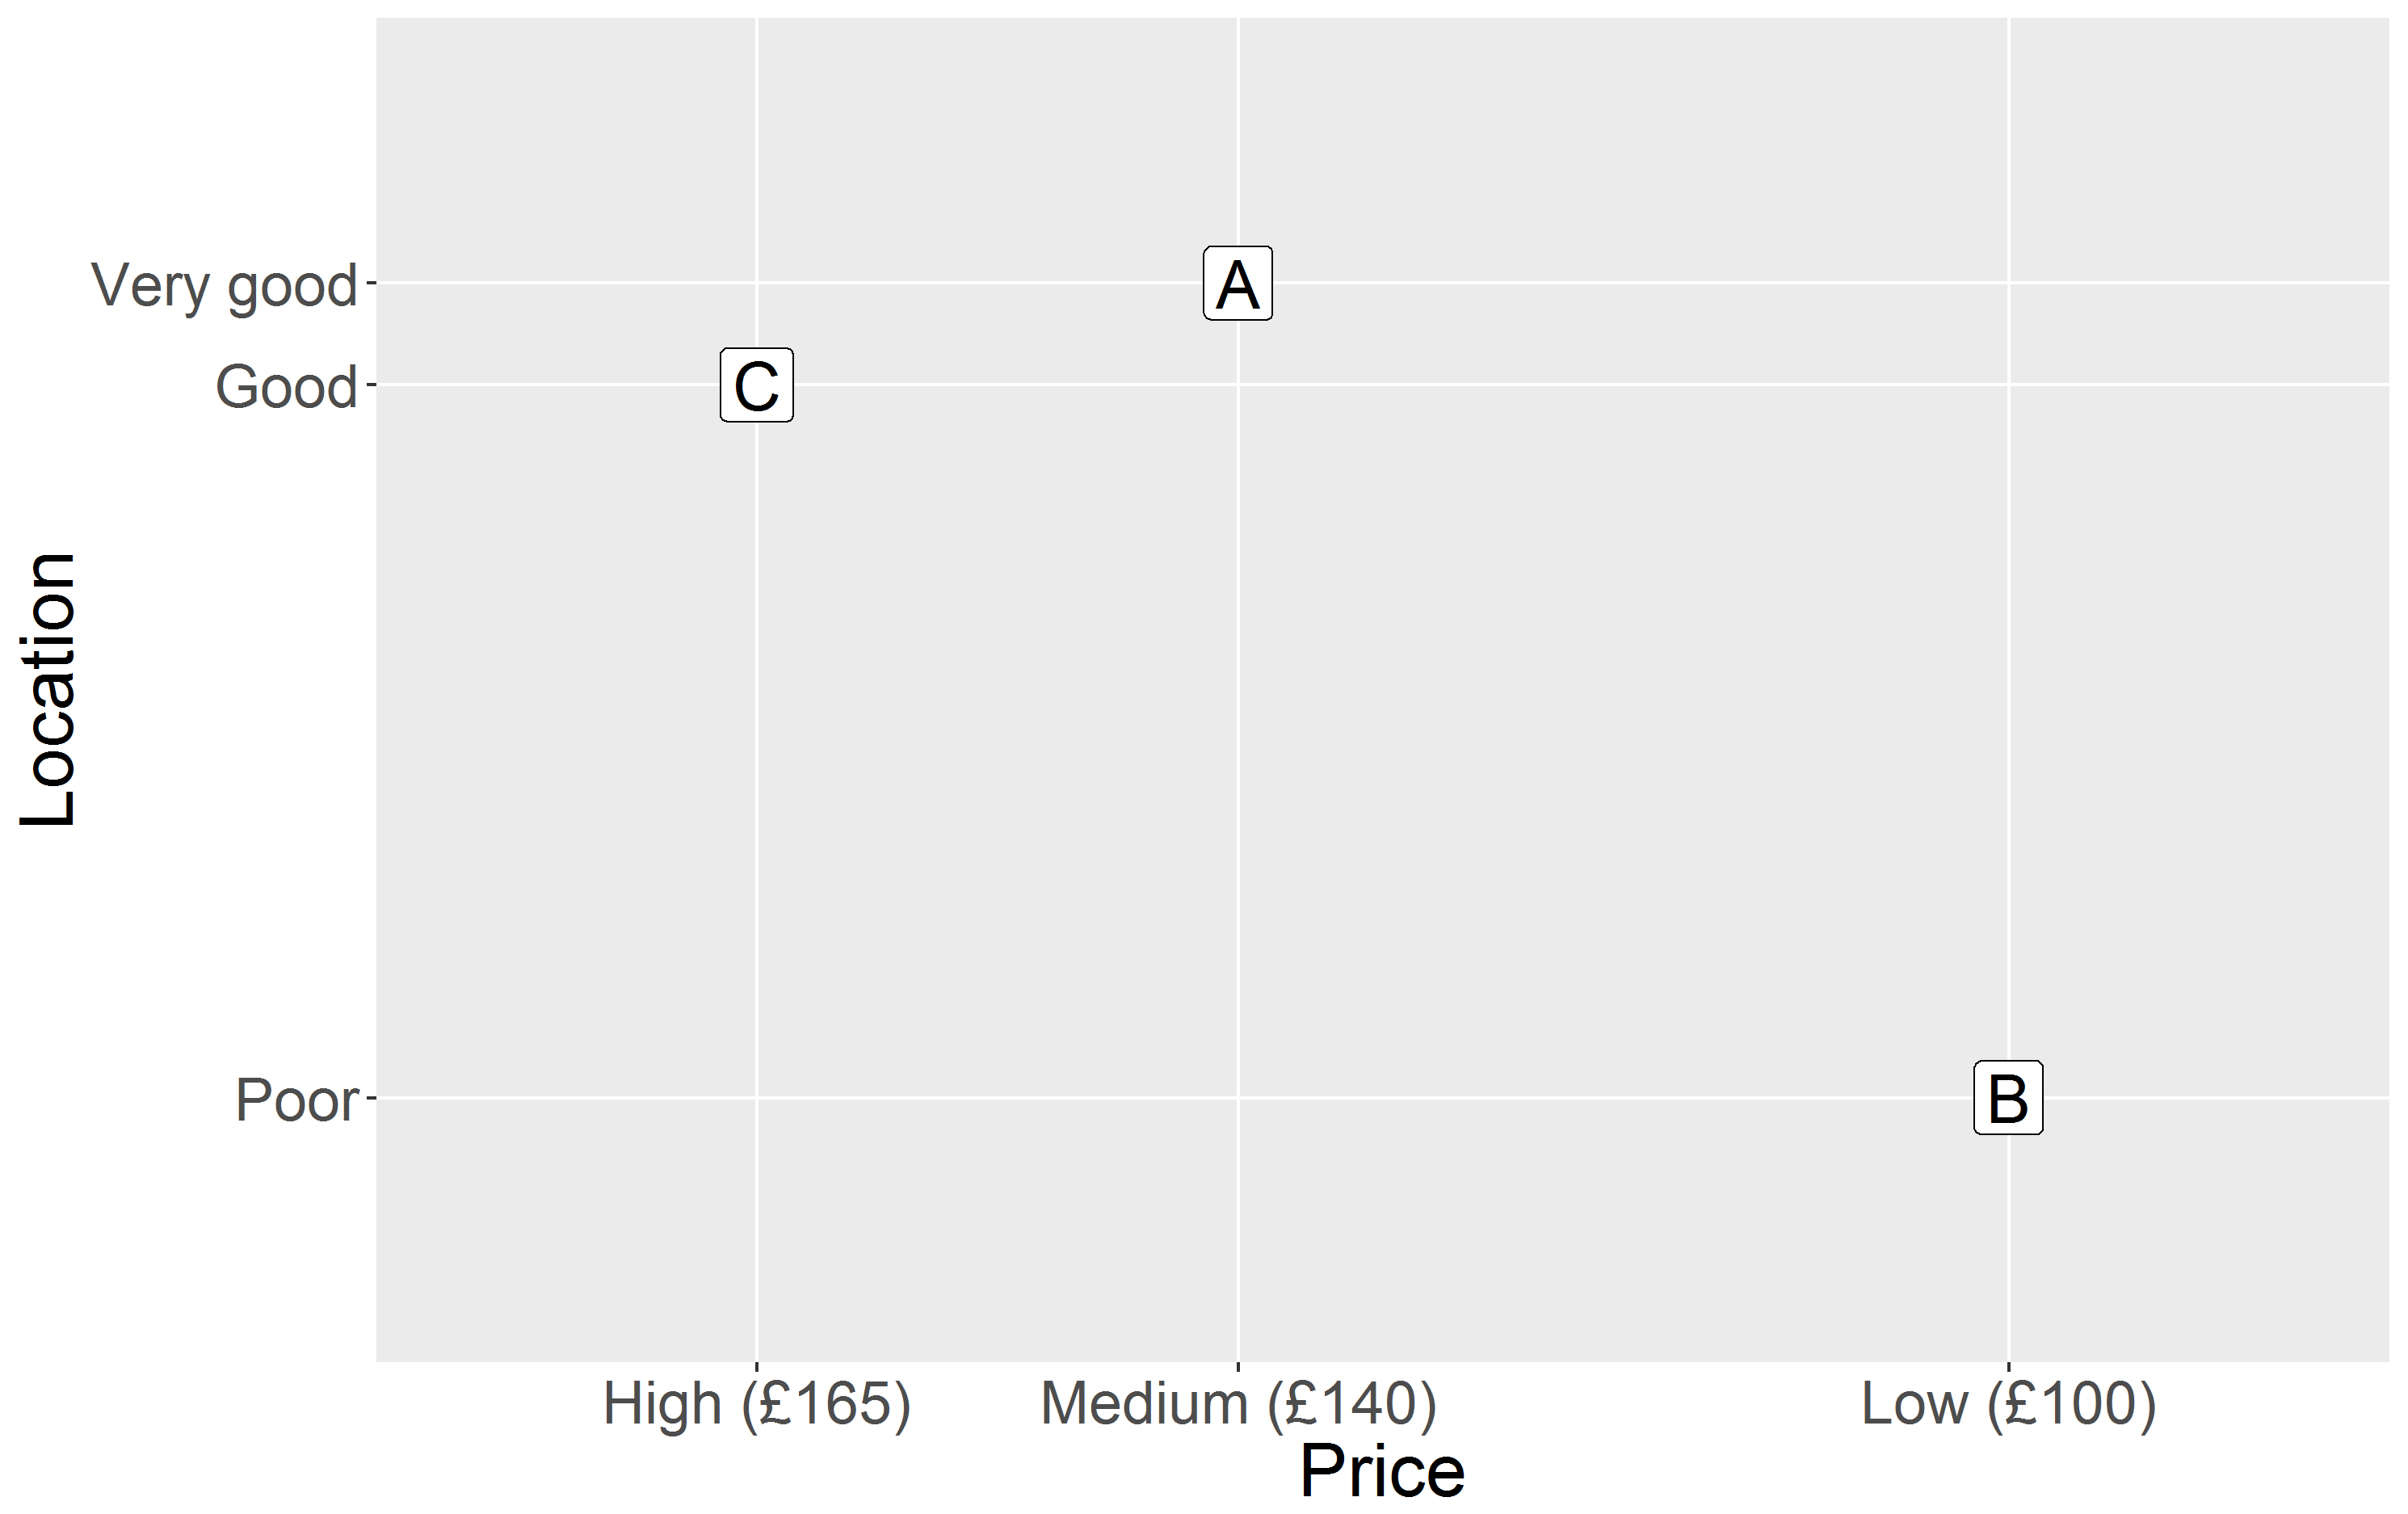
\includegraphics[width=0.8\textwidth]{exp1_intro.png}
\label{fig:exp1_intro}
\end{figure}

This effect poses a challenge to all choice models that rely on the assumption that preferences can be represented on a cardinal scale in the form of utilities (this is also called simple scalability, one of the consequences of Luce's Choice Axiom \cite{Luce1959}. Such models must also satisfy two axioms. 
The first is called order independence (its stricter version is known as independence from irrelevant alternatives), which requires that the preference ranking of two options should not be affected by adding new options to the choice set. The second axiom is called regularity, and it states that by extending the choice set, an option's choice probability cannot increase (\citeNP{Luce1977}; \citeNP{Tversky1972a}).

The attraction effect clearly violates these axioms, as it shows that the addition on an inferior decoy option increases the preference for the target over the competitor. This means that preferences for one option cannot be represented by a single internal magnitude that is invariant to the other options' value in the choice set. In fact, the presence of the effect points to a choice model where the preference for a choice option is strongly affected by the range of available options through the comparison process.

The attraction effect has been studied extensively over the past few decades using various experimental populations and conditions, as well as stimuli types. This research had shown that older adults are less susceptible to this decision bias compared to young adults \cite{Kim2005}, and that children as young as 5-year-old already exhibit this effect \cite{Zhen2016}. 

Several studies have investigated whether such choice biases are also present in animal decision-making. This line of research is very important as it has the potential to deliver valuable insights into the evolutionary origins of the attraction effect and related choice biases, informing attempts to model human decision-making. Unfortunately, results from this area so far seem fairly inconclusive. While decoy effects have been observed in various animals from brainless amoebas \cite{Latty2011}, to honeybees, grey jays \cite{Shafir2002} and rhesus macaques \cite{Parrish2015}, a similar number of studies report conflicting results (in rhesus macaques, \citeNP{Parrish2018}; capuchin monkeys, \citeNP{Cohen2017}; ant colonies, \citeNP{Edwards2009}; and hummingbirds, \citeNP{Bateson2002}). 

It is possible that there is no single, coherent explanatory framework for these results, as the aforementioned studies have utilized a wide range of experimental tasks and used very different subject populations, thus they might only be superficially similar. In any case, these inconclusive results point out the attraction effect's sensitivity to the experimental task and population, and stresses  the importance of exploring the boundary conditions of the effect. 


In humans, the strength of the effect has been probed under various experimental conditions. Research in this area have shown that the attraction effect is more pronounced under time pressure \cite{Pettibone2012}, and less pronounced with undesirable choice options \cite{Malkoc2013}, and feedback after choice \cite{Ahn2015}. \citeA{Mao2012} found that the strength of the effect is also influenced by individual differences: in their experiment, people who relied more on intuitive reasoning showed a stronger attraction effect. 


The role of individual heterogeneity has also been the focus of recent research that attempted to accommodate the three most well-known decision biases (the attraction, similarity, and compromise effects, also known as the Big Three) in a single modelling framework. A meta-analysis by \textcolor{red}{Tsetsos et al (can't find it on google scholar just yet)} has found that while the size of the attraction and compromise effects are positively correlated, both are negatively correlated with the size of the similarity effect. A recent study by \textcolor{red}{Cataldo} offers a simple, plausible explanation for this finding. 

In this study, they manipulated the presentation format of the choice options (such that the presentation format facilitated either an alternative-wise or an attribute-wise comparison process), and found that the attraction and compromise effects were stronger in the condition where participants were encouraged to use an attribute-wise comparison process, whereas the similarity effect was stronger in the alternative-wise condition. This finding suggests that any modelling attempt that aims to offer an explanation for all three decision biases must take into account how individual heterogeneity affects the comparison strategy.


Several explanations have been put forward to explain the attraction effect. \citeA{Simonson1989a} proposed that the decoy makes it easier to justify the subsequent choice of the target. \citeauthor{Huber1982} suggested that the presence of the decoy changes the reference level against which the target and the competitor are evaluated, making the target seem relatively more attractive. With the added assumption of loss aversion, prospect theory also uses reference-dependence to explain the attraction effect \cite{Sivakumar2016}. Another explanation that had been proposed is trade-off aversion (e.g., \citeNP{Hedgcock2009}). According to this theory, the attraction effect stems from the decision maker's inherent desire to avoid negative emotion. This is because the presence of the decoy reduces the cognitive cost and any potential negative affect generated during the evaluation and subsequent comparison of two distinctly different choice options. 


The latest modelling efforts aiming to explain the attraction effect almost exclusively focused on sequential sampling models of choice. These models view the choice as a series of noisy evidence accumulation steps in favour of each choice option, where the option that first reaches a given threshold will be chosen. Prominent examples of these kind of models are multialternative decision field theory (MDFT, \citeNP{Roe2001}), multi-attribute decision by sampling (MDbS, \citeNP{Noguchi2014}), the leaky competing accumulator model (LCA, \citeNP{Usher2004}), the multiattribute linear ballistic accumulator model (MLBA, \citeNP{Trueblood2014}), and the associative accumulation model (\citeNP{Bhatia2013a}). 

These sequential sampling models became very popular in decision making research since they can explain the attraction effect along with other well-documented decision biases in a single modelling framework. While the models listed above share the same sequential sampling principle, they rely on different assumptions in explaining the attraction effect. Specifically, the MDFT sees the attraction effect as a result of the inhibitory links between alternatives, the LCA relies on loss aversion and inhibition, the MDbS assumes changes in the distribution of the evidence samples, the MLBA explains the attraction effect using the assumption of attention weights that are inversely proportional to the discriminability of two options, while the associative accumulation model produces the attraction effect through the increased accessibility of the attribute on which the target option is the strongest.

Considerable research has focused on the neural mechanism underlying the attraction effect. These studies have typically used functional resonance imaging (fMRI) to measure neural activity during choice, and had shown that neural activation in certain brain regions depend on the relative value of the option under consideration in the current choice context (e.g., \citeNP{Mohr2017}; \citeNP{Chung2017}; \citeNP{Gluth2017}). These studies also lend support to models that utilize a sequential sampling principle, as neural activity during choice in brain regions that are involved in decision making (specifically, in certain prefrontal and parietal cortical areas) often resemble an accumulation process (\textcolor{red}{Busemeyer et al}). Most importantly, results from studies that use neural recordings support the view that value is constructed and therefore is intrinsically dependent on the context.


\subsection{The real-world relevance of the attraction effect}

The real-world relevance of the attraction effect has recently become a contentious issue in the decision-making literature. While the effect has previously been demonstrated over several choice domains (e.g., consumer products, \citeNP{Doyle1999}; medical decisions, \citeNP{Schwartz1999}; mate choice, \citeNP{Sedikides1999}; hiring decisions, \citeNP{Highhouse1996}; political choice, \citeNP{SueOCurry1995}; work-family benefits, \citeNP{Reb2018}; intertemporal choice, \citeNP{Gluth2017}; perceptual decisions, \citeNP{Trueblood2013}), and has recently been successfully used as a real-world nudge \cite{Li2018}, some claim that the attraction effect is much less prevalent in natural contexts than previously thought.

In their study, \citeA{Frederick2014} present a thorough investigation of the boundary conditions of the attraction effect based on 38 experiments with various stimuli types. These stimuli types include choice options with numerically represented attributes as well as complex, real-world stimuli (e.g., fruits, bottled water, apartments, etc.), and  in some of these experiments participants could even sample the choice options (e.g. squash, mints, popcorn). The overall conclusion of this study is that while the presence of the decoy seems to affect decisions when the option attributes are represented numerically, it is absent in experiments with more complex, naturalistic stimuli. In light of these results, \citeauthor{Frederick2014} posited that the psychological processes underlying decisions that involve options with numeric attributes are fundamentally different from those employed in decisions where the stimuli has a naturalistic representation. This conclusion was also supported by \citeA{Yang2014}, who reported difficulties replicating the attraction effect when the stimuli were pictorial, as opposed to when attributes were presented numerically.


These two studies sparked considerable interest amongst decision making researchers, and led to the re-examination of the boundary conditions of the attraction effect. \citeA{Huber2014} discussed five critical conditions that can inhibit the attraction effect, and argued that many of these are present in the experiments reported by \citeauthor{Frederick2014} and \citeauthor{Yang2014}, which can explain their failure to observe the effect. These are the following: (1) strong prior preferences over the target and competitor, (2) inability to identify the inferiority of the decoy, (3) heterogeneity in prior preferences over the target and competitor, (4) an undesirable decoy and (5) a too desirable decoy. \citeA{Simonson2014a} further stressed the importance of the detection of the dominance relationship in observing the attraction effect, and also pointed out several other smaller, specific methodological shortcomings of the studies by \citeauthor{Frederick2014} and \citeauthor{Yang2014}. 

%Joining this debate, \citeA{Lichters2015a} listed a number of factors that increase the likelihood of observing the attraction effect. These include choices with real economic consequences, realistic product representation, the presence of a no-buy option, participants who are interested in the product, and the possibility of a sensory evaluation of the choices.

While these reactions have seemingly ended the debate, we believe that the literature  is still lacking a conclusive answer regarding the presence of the attraction effect in choices with non-numeric option attribute presentations. A rigorous investigation of this question would not only inform us about the real-world relevance of the attraction effect, but would also shed light on the commonalities between the cognitive mechanisms underlying choices that involve options with numeric and naturalistic attributes.


In light of the conflicting views about the importance of this effect, this study is an attempt to replicate the attraction effect using naturalistic stimuli with non-numeric attributes, whilst accounting for the major concerns raised in connection with \citeauthor{Frederick2014} and \citeauthor{Yang2014}'s studies. Specifically, our novel experimental design ensures that decision makers are indifferent between the target and competitor and that the inferiority of the decoy is clearly identified. In addition, to increase the statistical power of our test, we used a within-subjects design to identify the effect as well as both A, B, A' and B, A, B' triplet pairs, where X' is the dominated option (as suggested by \citeNP{Huber2014}). 

\subsection{Overview of Experiment 1 and 2}

When selecting the type of naturalistic stimuli for testing the attraction effect, our decision was guided by a few simple criteria we considered important for creating target-decoy-competitor triplets. First, we needed a stimuli that would be at least of some interest to most people, or at least would be familiar to most of our participants. Second, the stimuli needed to have multiple attributes, which can take a wide variety of values, as most real-world stimuli does. Third, we needed to be able to establish the degree of similarity between pairs of items, which is a non-trivial task in the case of naturalistic stimuli, due to the potentially high number of dimensions and their incommensurability. In addition, we also needed a large number of items to create enough triplets for a powerful within-subjects design. 


We decided to use movie posters as stimuli, as it satisfied most of our criteria. Movies are an integral part of popular culture in Western societies, thus we could reasonably expect that most participants will be familiar with well-known movies. They also vary greatly by genre and topic, which offers us a natural way to establish similarity between pairs of movies. In addition, even if we only use reasonably well-known movies, we still have a vast pool of items to create triplets from.


When choosing between naturalistic items such as movies, the decision maker cannot rely on the numerical attributes of the choice options to establish similarity and build a preference ordering (strictly speaking this is not true in a non-experimental context, where people can always at least partly base their decision on the numeric rating of the movie, but this information was not available in our experiment). We expect mnemonic processes to have a very important role in building preference representations of movie items, and while this is inevitable if we are to use complex items that people are familiar with, it can also be potentially problematic. Specifically, we do not exactly know how the retrieval and preferences construction process works and the extent to which individual heterogeneity affects it.

However, regardless of how the preference representations are constructed, we expect the comparison process to take place along a few salient attribute dimensions. For example, these dimensions are likely to include the story themes, the genre of the movie, and perhaps the actors and director. Therefore, it is possible to establish a method to create movie pairs that are likely to be perceived different or similar, using all available information on these movies.

In Experiment 1, we used two criteria to establish a measure of similarity between our naturalistic stimuli items. First, we used latent semantic analysis on the text associated with each movie (including various descriptions of the movie as well as the information on the actors and director). Section  \ref{lsa_description} provides a brief overview of what latent semantic analysis entails. Second, we used the overlap in genre categories that movies were assigned to on IMDb as a measure of similarity. 

We did not find any evidence for the attraction effect in Experiment 1, but the results also indicated that the perceived similarity between the target and decoy movies were often not strong enough to consider this as a valid test of the attraction effect. Therefore, in Experiment 2, we relied on more detailed genre information from allmovie.com, as well as similarity ratings from an independent experiment to establish similarity. The target-decoy pairs were indeed perceived as more similar in Experiment 2, but we still did not find any evidence for the attraction effect. We speculate that this result arises from differences in cognitive processes underlying the evaluation of stimuli with numeric attributes versus naturalistic objects and discuss the implications of our findings.

\subsection{Establishing complex object similarity: latent semantic analysis} \label{lsa_description}


Latent semantic analysis (LSA; also known as latent semantic indexing) is a statistical technique that was developed in the 1990s as a novel method for automatic indexing and retrieval of text documents \cite{Deerwester1990}. 
In LSA, each document in a set is considered as a bag of words (a document here refers to a body of text). Thus the raw data for analysis are huge document-by-word matrices, where entries indicate the presence of a word in a document. Based on these matrices, the LSA algorithm builds a specified number of "latent dimensions", each of which can be represented with a set of words that reflects a common underlying theme in the documents. Then, similarity between any two documents can be established based on the overlap in the latent dimensions that best characterise them. This technique relies on singular value decomposition (SVD), a statistical tool that uses dimensionality reduction to build a simpler, approximate representation of a matrix \cite{Leskovec2014}. This tool underlies many real-world applications, from image compression to solving systems of linear equations (e.g., \citeNP{Akritas2004}). 

Enormous volumes of text data are being generated by users every day, and there is an increasing need to understand the underlying patterns in these texts. One of the most popular techniques used to achieve this is LSA. Accordingly, it has recently gained substantial popularity as a machine learning technique that had been used in various "big data" contexts, from predicting sales performance of movies from online reviews \cite{Yu2012} to building recommendation systems (e.g. \citeNP{Wu2008}), predicting political orientation from Twitter data \cite{Conover2011}, and detecting online bullying \cite{Bigelow2016}. Our research project largely builds on a study by \citeNP{Bhatia2018}, where they successfully used LSA to build multiattribute representations of choice options and predict subsequent choice behaviour.


To explain how the algorithm works in a nutshell, imagine that we have a set of movies (these are the documents) with the corresponding user-generated text that summarizes each movie. Then, we can create a so-called term-document matrix, where each row corresponds to a unique word found in these reviews, the columns are the movies itself, and the cells represent the number of times each word has appeared in a given movie description. We can call this matrix $M_{\text{TxD}}$, where T is the number of unique words that can be found in our corpus (the rows) and D is the number of movies (the columns). Say we are interested in retrieving k < min\{T,D\} underlying dimensions from these movie description texts, where k is a measure of the crudity of our simplified representation of these movies: the higher it is, the more detailed our alternative representation of matrix M, but the less efficient it is. 

Then, by performing a SVD, we can decompose matrix M the following way:

\begin{equation}
M_{TxD}=U_{Txk}\Sigma_{kxk}V_{kxD}
\label{eq:1}
\end{equation}

where $U_{Txk}$ is a matrix with the loading of each unique word on the underlying k latent dimensions. To put it differently, it contains information about the words that best describe the retrieved latent dimensions, giving interpretable meaning to them. Similarly, $V_{kxD}$ contains the loading of each document on these $k$ latent dimensions. One can consider the $V_{kxD}$ matrix as giving the coordinates of all of the movies in $k$-dimensional movie space, where $U_{Txk}$ defines each of the dimensions. The $k$ latent dimensions are always retrieved in their order of importance, defined by the share of variance they can explain (thus increasing the number of latent dimensions has a decreasing marginal return in terms of variance explained). Having obtained these matrices, we are ready to 1) describe each movie based on the latent dimensions it has the highest loading on and 2) establish similarity between the movies based on their common topics. Section \ref{choice_selection} demonstrates these steps using our movie stimuli.


\section{Experiment 1} 

\subsection{Method} \label{method_1}

\subsubsection{Stimuli}

As mentioned above, our aim was to select a rich set of movies as stimuli. To this end, we collected data from www.imdb.com on the most popular (given by the number of votes) 800 movies from each of the following genre categories: comedy, sci-fi, horror, romance, action, thriller, drama, mystery, crime, animation, adventure, fantasy; amounting to 9,600 movies overall. Since most movies appear in multiple categories, if a movie in one category has already been retrieved as part of another category the code continued to the next movie (the retrieval by category happened in the same order as they are listed above). The information we retrieved for each movie were the following: poster image, title, director, actors, number of votes, genre categories, plot keywords and summaries of the movie. Keywords and summaries describe the plot of the movie and are both generated by the users. We used both texts to establish semantic similarity between the movies.


 Before performing the LSA, the texts needed to be cleaned. This included removing any text that were not written in English, removing numbers, stop words, punctuation and duplicate words. In addition, we eliminated whitespace from keyword expressions that consisted of multiple words, and thus were treated as one word, to retain their meaning (e.g., expressions like "organized crime"). If, after these transformations, there were no text left for a given movie, it was excluded form the analysis. We had text data with 61,525 unique words for 9,272 movies.
 
 
 The next step was to create a term-document matrix with each row as a word and each movie as a column. We then used term frequency-inverse document frequency weighting (also known as tf-idf) to measure the importance of each word in each movie text. Assuming that there are $i = 1...T$ rows (words) and  $j = 1...D$ columns (movies), and $n_{i,j}$ is the number of times a word occurs in a given document, we applied the following weight to each cell:
 
 \begin{equation}
weight_{i,j}=\frac{n_{i,j}}{\sum_{i=1}^{T} n_{i,j}}\log{\left(\frac{D}{\sum_{j=1}^{D} \min\{n_{i,j},1\}}\right)}
\end{equation}
 
 In other words, for a given word and document, the weight is the product of the 1) share of the word from all the words in that document multiplied with the logarithm of 2) the overall number of documents divided by the number of documents that contain the word.  
  
  The underlying principle of this weighting scheme is that the importance of a term is inversely proportional to the number of documents it appears in. For example, "murder" and "kamikaze" are both keywords used to describe the plot of Pearl Harbor, but since "murder" appears in 3,336 movie descriptions whereas "kamikaze" only appears in 10, the latter is assumed to contain more information about the movie, and therefore will be assigned a higher weight. We performed the latent semantic analysis on this cleaned, weighted corpus.


\subsubsection{Choice set selection} \label{choice_selection}

We decided to use a latent semantic solution with 20 latent dimensions, as we found that this number gives us a sufficiently rich latent dimension space to establish similarity between movies, while keeping computational complexity at a reasonable level. Figure \ref{fig:latentdims} shows the 10 first words with the highest absolute loading on these 20 dimensions (this is part of the $U_{Txk}$ matrix from Equation \ref{eq:1}). Words that have an orange colour load positively on the given dimension, while words in blue load negatively on them. This means that some of the dimensions have a somewhat counterintuitive "reversed definition", and are described by words that are the \textit{least} characteristic of them. 

For example, the words that best describe latent dimension number 4 are "slasher", "maniac", "homicidal maniac", which all relate to a serial killer story, so we would expect serial killer movies to load highly on this dimension, whereas movies with no such theme (e.g., romantic comedies) to load negatively on this dimension. Similarly, latent dimension number 5 has high negative loadings for words that relate to interpersonal relationships, such as "marriage", "romance", "married", so we would expect romantic movies to load negatively on this dimension (as the dimension can be best described as "non-romantic"), whereas any movie without such themes (e.g. animated superhero movies, zombie movies) should load positively on this dimension. 

Table \ref{tab:movies_desc} shows the ranking of the 20 latent dimensions for four selected movies. The ranking is based on the absolute value of the movie's loading on a given dimension (this was derived from matrix $V_{kxD}$ from Equation \ref{eq:1}), such that the latent dimensions are listed in descending order of relevance for each movie. Similarly to Figure \ref{fig:latentdims}, the colour code shows the direction of the association: the dimension number is coloured orange if the movie loads positively on that given dimension, and blue if it loads negatively.

 Based on the information presented in Figure \ref{fig:latentdims} and Table \ref{tab:movies_desc}, we can now attempt to describe each of the four movies based on what the algorithm tells us about them. Naturally, dimensions with positive loadings are more helpful if one wishes to use the latent semantic solution to build a lower-level representation of each movie. For example, assuming no prior knowledge about these four movies, the latent semantic analysis solution tells us that Deadpool is a superhero movie with adult themes (such as nudity and violence), Love Actually is a movie set in the real world and is about romantic relationships, Psycho features homicide and is set in the US countryside, while Wolf of Wall Street is a movie that is set in the US with lots of adult scenes (mostly sexual, but there is violence too) that features an investigation. 
 
 While even a human might find it hard to accurately describe a large, diverse set of movies with only 20 "themes", the algorithm seems to perform surprisingly well in capturing the most important aspects of these movies, highlighting the efficacy of the LSA algorithm. 

\newcounter{savepage}
\cleardoublepage
\setcounter{savepage}{\arabic{page}}
\newgeometry{left=5cm,bottom=2cm, right = 2cm, top = 1cm}
\begin{landscape}
\pagenumbering{gobble}
\begin{figure}
\captionsetup{justification=centering}
\caption{The ten most important terms (with the highest absolute loading) for each of the 20 latent dimensions. Orange coloured terms load positively on the latent dimensions, whereas blue coloured terms load negatively on the dimensions.}
\centering
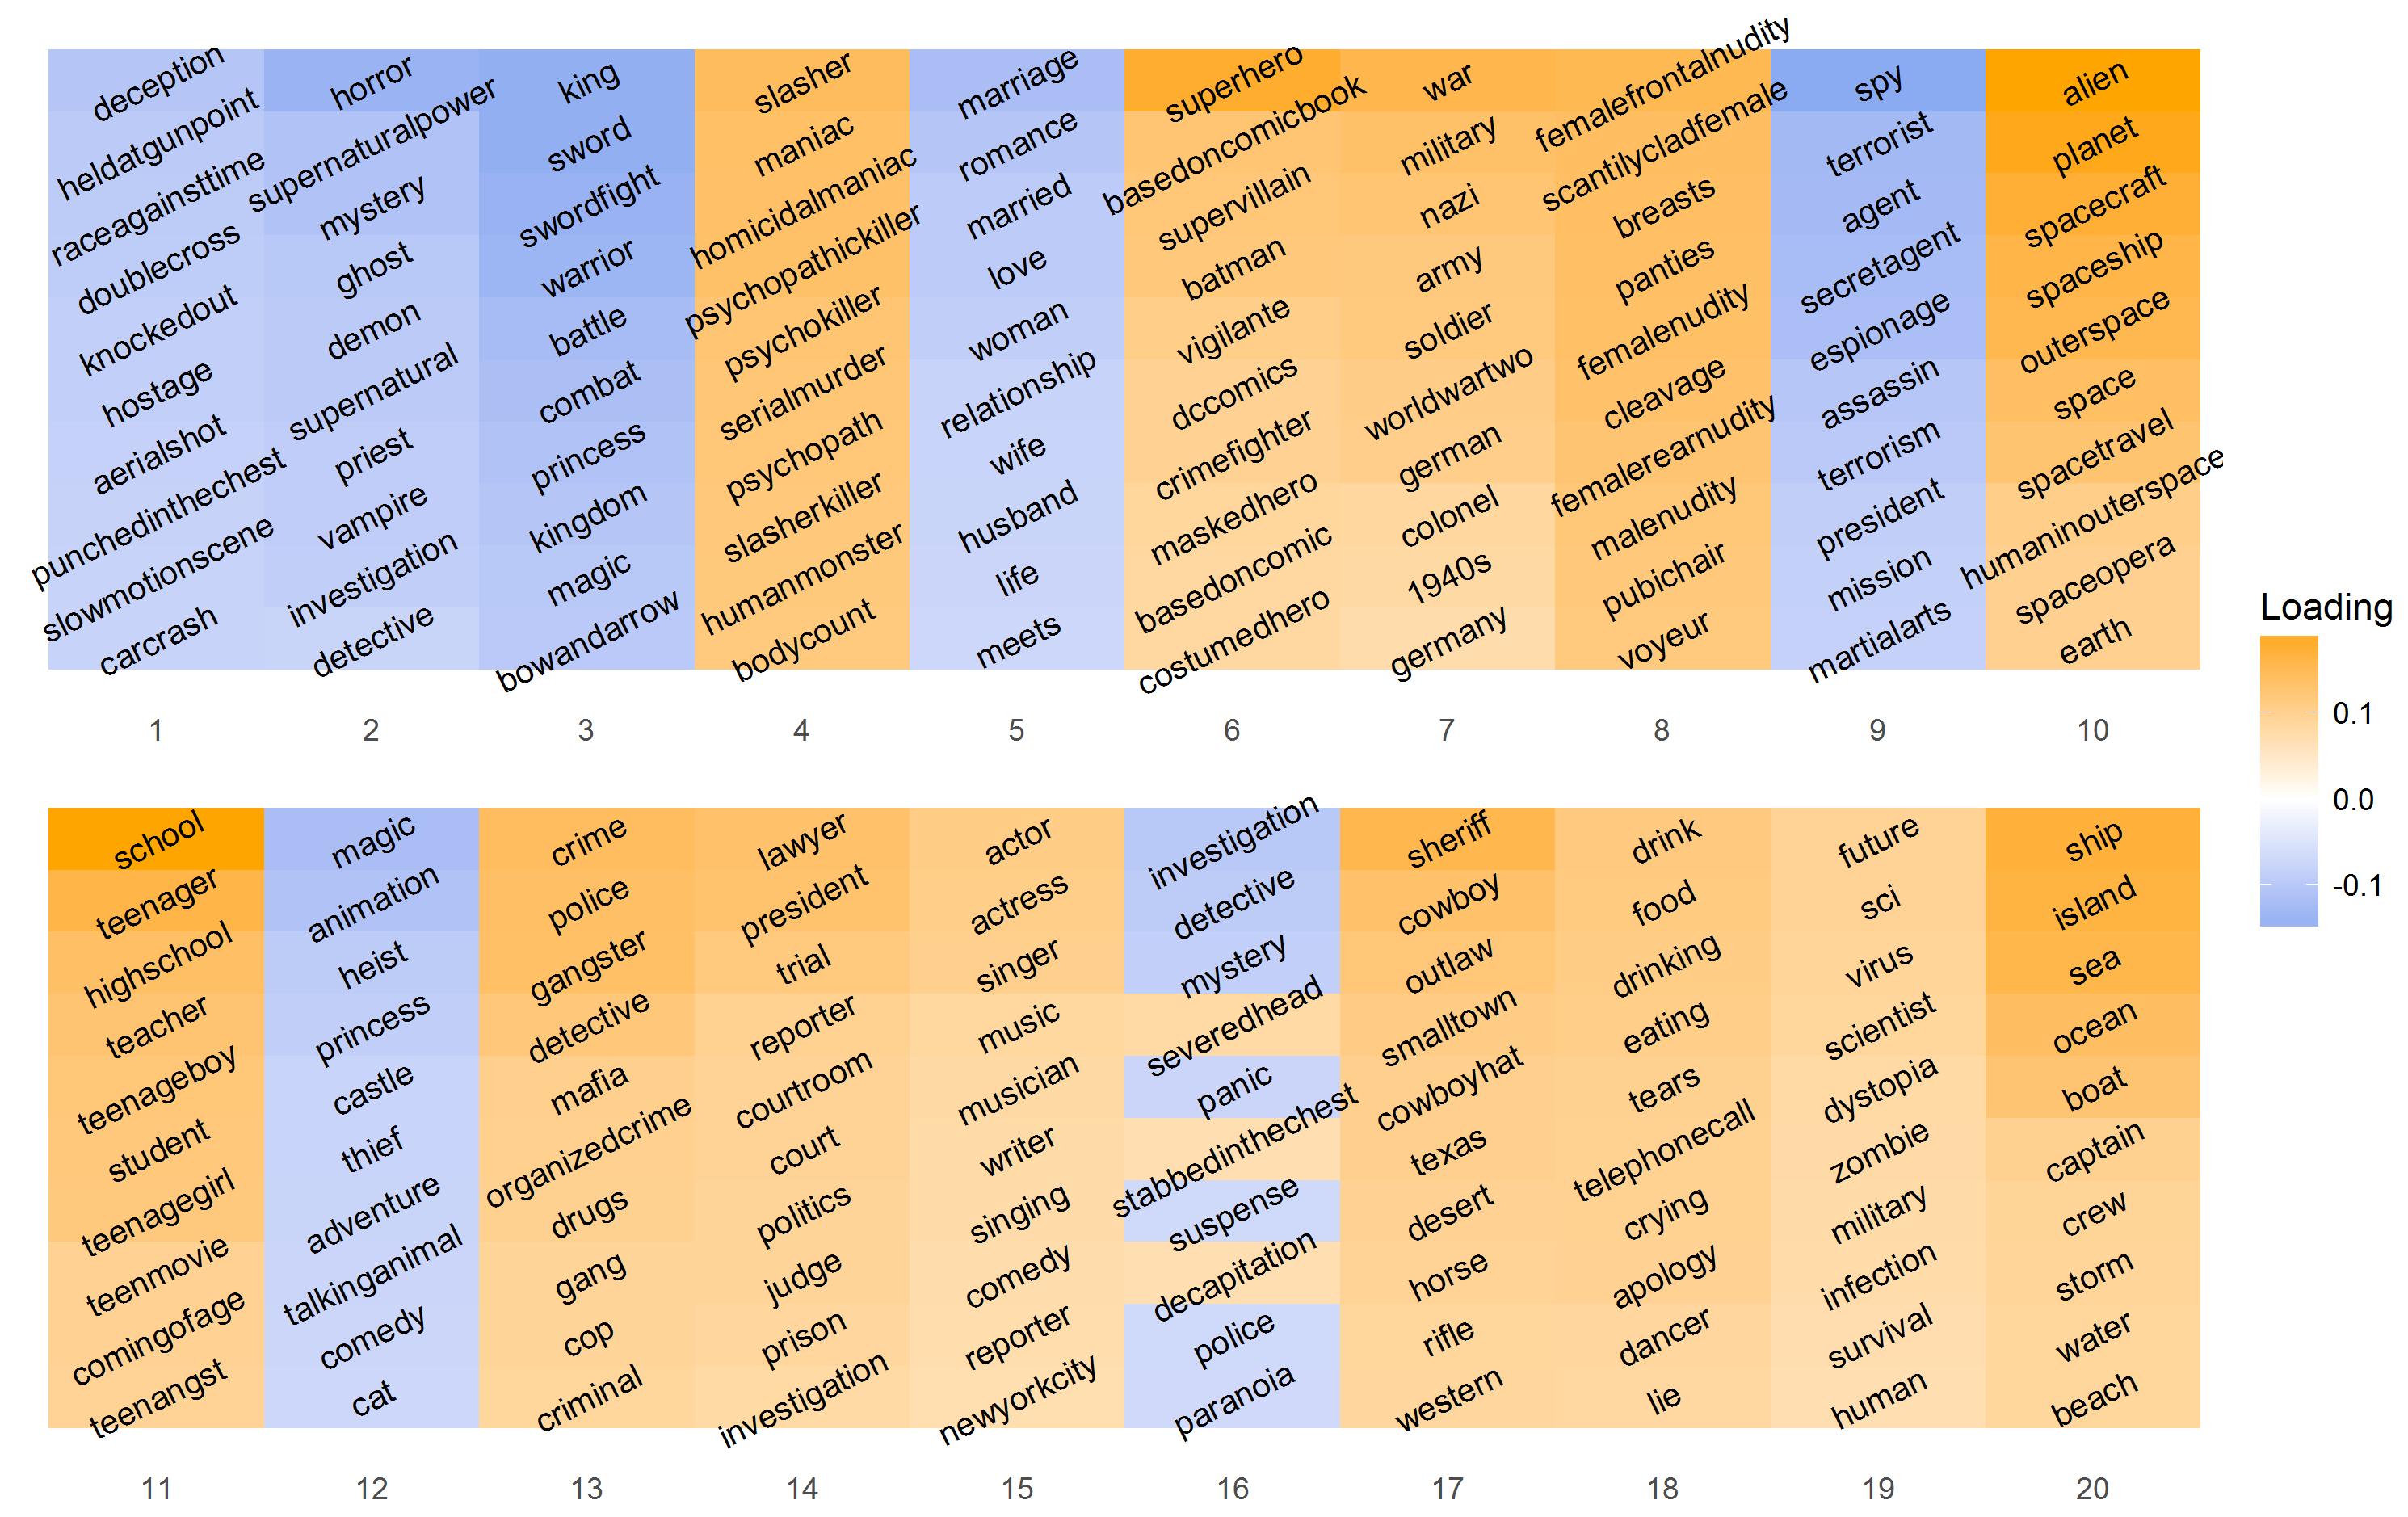
\includegraphics[width=1.45\textwidth]{latent_dims.png}
\label{fig:latentdims}
\end{figure}
\end{landscape}
\restoregeometry
\cleardoublepage
\pagenumbering{arabic}
\setcounter{page}{\thesavepage}

%A: It looks quite crammed when I try to represent it as a table (because we have 20 dimensions, and some of the words are just too long). I think the graphical aspect helps the reader to quickly understand what the dimensions mean by referring to the colours, without displaying exact loading value, which is not crucial info (I think only relative magnitudes and sign matters - both of which are captured by the colour code.


\begin{table}[H]
\captionsetup{justification=centering}
\caption {Ranking of the 20 latent dimensions for each of the four selected movies (based on the movies' absolute loading on each dimension), in descending order of relevance. The movies load positively on orange coloured latent dimensions, and negatively on blue coloured dimensions.} \label{tab:movies_desc} 
\resizebox{\columnwidth}{!}{\begin{tabular}{>{\centering\arraybackslash}m{3cm}>{\centering\arraybackslash}m{3cm}>{\centering\arraybackslash}m{3cm}>{\centering\arraybackslash}m{3cm}>{\centering\arraybackslash}m{3cm}}
\toprule
\textbf{Rank} & \textbf{Deadpool} & \textbf{Love Actually} & \textbf{Psycho} & \textbf{The Wolf of Wall Street}\\
\midrule
1 & \color{orange}{ 6 } & \color{orange}{ 15 } & \color{orange}{ 4 } & \color{orange}{ 14 }\\
2 & \color{orange}{ 16 } & \color{blue}{ 5 } & \color{blue}{ 5 } & \color{orange}{ 8 }\\
3 & \color{blue}{ 1 } & \color{orange}{ 8 } & \color{orange}{ 17 } & \color{orange}{ 20 }\\
4 & \color{orange}{ 12 } & \color{blue}{ 13 } & \color{orange}{ 2 } & \color{orange}{ 16 }\\
5 & \color{blue}{ 7 } & \color{orange}{ 12 } & \color{blue}{ 16 } & \color{blue}{ 19 }\\
\addlinespace
6 & \color{orange}{ 8 } & \color{orange}{ 14 } & \color{blue}{ 11 } & \color{blue}{ 7 }\\
7 & \color{blue}{ 14 } & \color{orange}{ 2 } & \color{blue}{ 12 } & \color{orange}{ 15 }\\
8 & \color{blue}{ 10 } & \color{blue}{ 1 } & \color{blue}{ 13 } & \color{blue}{ 1 }\\
9 & \color{orange}{ 19 } & \color{blue}{ 19 } & \color{blue}{ 19 } & \color{orange}{ 18 }\\
10 & \color{orange}{ 15 } & \color{blue}{ 11 } & \color{blue}{ 7 } & \color{blue}{ 17 }\\
\addlinespace
11 & \color{blue}{ 20 } & \color{blue}{ 20 } & \color{orange}{ 14 } & \color{orange}{ 2 }\\
12 & \color{blue}{ 5 } & \color{orange}{ 18 } & \color{orange}{ 10 } & \color{orange}{ 5 }\\
13 & \color{blue}{ 3 } & \color{blue}{ 9 } & \color{orange}{ 3 } & \color{blue}{ 11 }\\
14 & \color{blue}{ 13 } & \color{orange}{ 17 } & \color{orange}{ 15 } & \color{blue}{ 3 }\\
15 & \color{orange}{ 4 } & \color{blue}{ 6 } & \color{blue}{ 8 } & \color{orange}{ 9 }\\
\addlinespace
16 & \color{blue}{ 9 } & \color{blue}{ 3 } & \color{blue}{ 20 } & \color{orange}{ 13 }\\
17 & \color{blue}{ 2 } & \color{blue}{ 10 } & \color{blue}{ 1 } & \color{orange}{ 6 }\\
18 & \color{blue}{ 11 } & \color{orange}{ 7 } & \color{blue}{ 6 } & \color{blue}{ 12 }\\
19 & \color{blue}{ 17 } & \color{blue}{ 4 } & \color{blue}{ 18 } & \color{orange}{ 10 }\\
20 & \color{orange}{ 18 } & \color{orange}{ 16 } & \color{blue}{ 9 } & \color{blue}{ 4 }\\
\bottomrule
\end{tabular}}
\end{table}

%A: I again omitted the exact values, as they don't really matter and make it harder interpret the table.


We used all 9,272 movies to build a latent semantic representation of the types of movies people encounter, but we only used 200 movies as stimuli in the experiment. These movies were chosen in the following way. We selected ten genres (romance, drama, sci-fi, thriller, comedy, horror, animation, fantasy, crime, action), and retrieved the first 20 most popular movies in each genre. This happened in a sequential manner, starting the retrieval with the genres with the lowest number of movies (the final order was horror, romance, animation, fantasy, comedy, thriller, crime, sci-fi, action, drama). The rationale behind this approach was to avoid having relatively unknown movies appearing in a category (in case the well-known ones have already been retrieved as part of another category). We excluded any movies that were part of a sequel if a member of that sequel has already been selected.




Once we knew each movie's loading on the 20 latent dimensions, we could calculate the Euclidean distance between any two of the 200 movies. Based on this calculation, Table \ref{tab:movies_closefurth} shows the closest (most similar) and furthest (least similar) five movies for another four selected movies (Interstellar, Inglourious Basterds, The Hobbit: An Unexpected Journey, Star Wars: Episode IV - A New Hope). 


This demonstrates that while the algorithm seems to perform well in finding common themes in movies (e.g., the space theme for Interstellar and Star Wars, the war theme for Inglourious Basterds, and the adventure in a magical world theme in The Hobbit), there are a few odd matches. In particular, two movies can have very similar themes, but they might fall into  two completely different genres, and thus would never be perceived as similar. A good example is the proximity of WALL-E and Interstellar: while both score high on the outer space theme, WALL-E is an animated family movie, while Interstellar is a sci-fi adventure movie, and therefore they are unlikely to be perceived as similar. Other odd matches include Interstellar - Alien and The Hobbit - Shrek, which further show that latent semantic proximity alone is not enough to create similar movie pairs.

\begin{table}[H]
\captionsetup{justification=centering}
\caption {Closest and furthest five movies for four selected movies based on the Euclidean distance calculated from the LSA solution.} \label{tab:movies_closefurth} 
\resizebox{\columnwidth}{!}{\begin{tabular}{c>{\centering\arraybackslash}m{3cm}>{\centering\arraybackslash}m{3cm}>{\centering\arraybackslash}m{3cm}>{\centering\arraybackslash}m{3cm}}
\toprule
\textbf{Target} & \textbf{Interstellar} & \textbf{Inglourious Basterds} & \textbf{The Hobbit} & \textbf{Star Wars}\\
\midrule
Closest 1 & Alien & Saving Private Ryan & Shrek & Star Trek\\
Closest 2 & Oblivion & Casablanca & The Lord of the Rings & Avatar\\
Closest 3 & WALL·E & The Pianist & Monty Python and the Holy Grail & Guardians of the Galaxy\\
Closest 4 & 2001: A Space Odyssey & Full Metal Jacket & Frozen & The Fifth Element\\
Closest 5 & Gravity & Schindler's List & Alice in Wonderland & Oblivion\\
\midrule
Furthest 5 & Titanic & Man of Steel & Man of Steel & Life of Pi\\
Furthest 4 & Deadpool & Star Trek & Star Trek & Watchmen\\
Furthest 3 & The Wolf of Wall Street & The Dark Knight & The Wolf of Wall Street & Deadpool\\
Furthest 2 & The Dark Knight & The Wolf of Wall Street & The Dark Knight & The Wolf of Wall Street\\
Furthest 1 & Star Wars & Star Wars & Star Wars & The Dark Knight\\
\bottomrule
\end{tabular}}
\end{table}


To mitigate this problem, we decided to also use a genre similarity criteria using the genre classification information we retrieved from IMDb. This classification contains at least one and at most three main genre types that best describe each movie's type. The simplest approach would be to calculate the number of overlapping genres and rank each movie pair based on this measure. However, there are two problems with this approach. First, the genres used in the IMDb classification are rather crude, since there are only about 18 main genre types. Second, many movies only have one genre assigned to it, decreasing the quality of the genre matching criteria. 

For this reason, we decided to use a different method to calculate the genre similarity between any two movies. Our method consists of three parts, each with a separate score, and the sum of these is the final score, reflecting the genre similarity between each movie pair. 

The first part of the score is simply the number of overlapping genres between the two movies. However, as we mentioned above, the genre information is rather scarce for many movies (although every movie has at least one genre), therefore we decided to use the concept of genre similarity as the second criterion. For example, considering a romance, thriller and horror movie, and assuming we do not have any additional genre information on these movies, we would naturally like the thriller and horror movies to be closer to each other than to the romance movie. 

To gauge the "proximity" of any two genres, we used genre information from all 9,272 movies in our database to build a genre correlation matrix, which reveals common "genre-mixtures" (see Figure \ref{fig:corr}), that often appear together in genre lists. Then, considering movie pair A and B, we can calculate the number of genres that are positively correlated with the main genre of movie A (the first genre in its genre list) and also appear in the genre list of movie B. For example, using this criteria, the thriller and horror movies would be closer to each other than to the romance movie, since thriller and horror are positively correlated with each other, and both are negatively correlated with romance. 


\begin{figure}
\caption{Genre correlation matrix.}
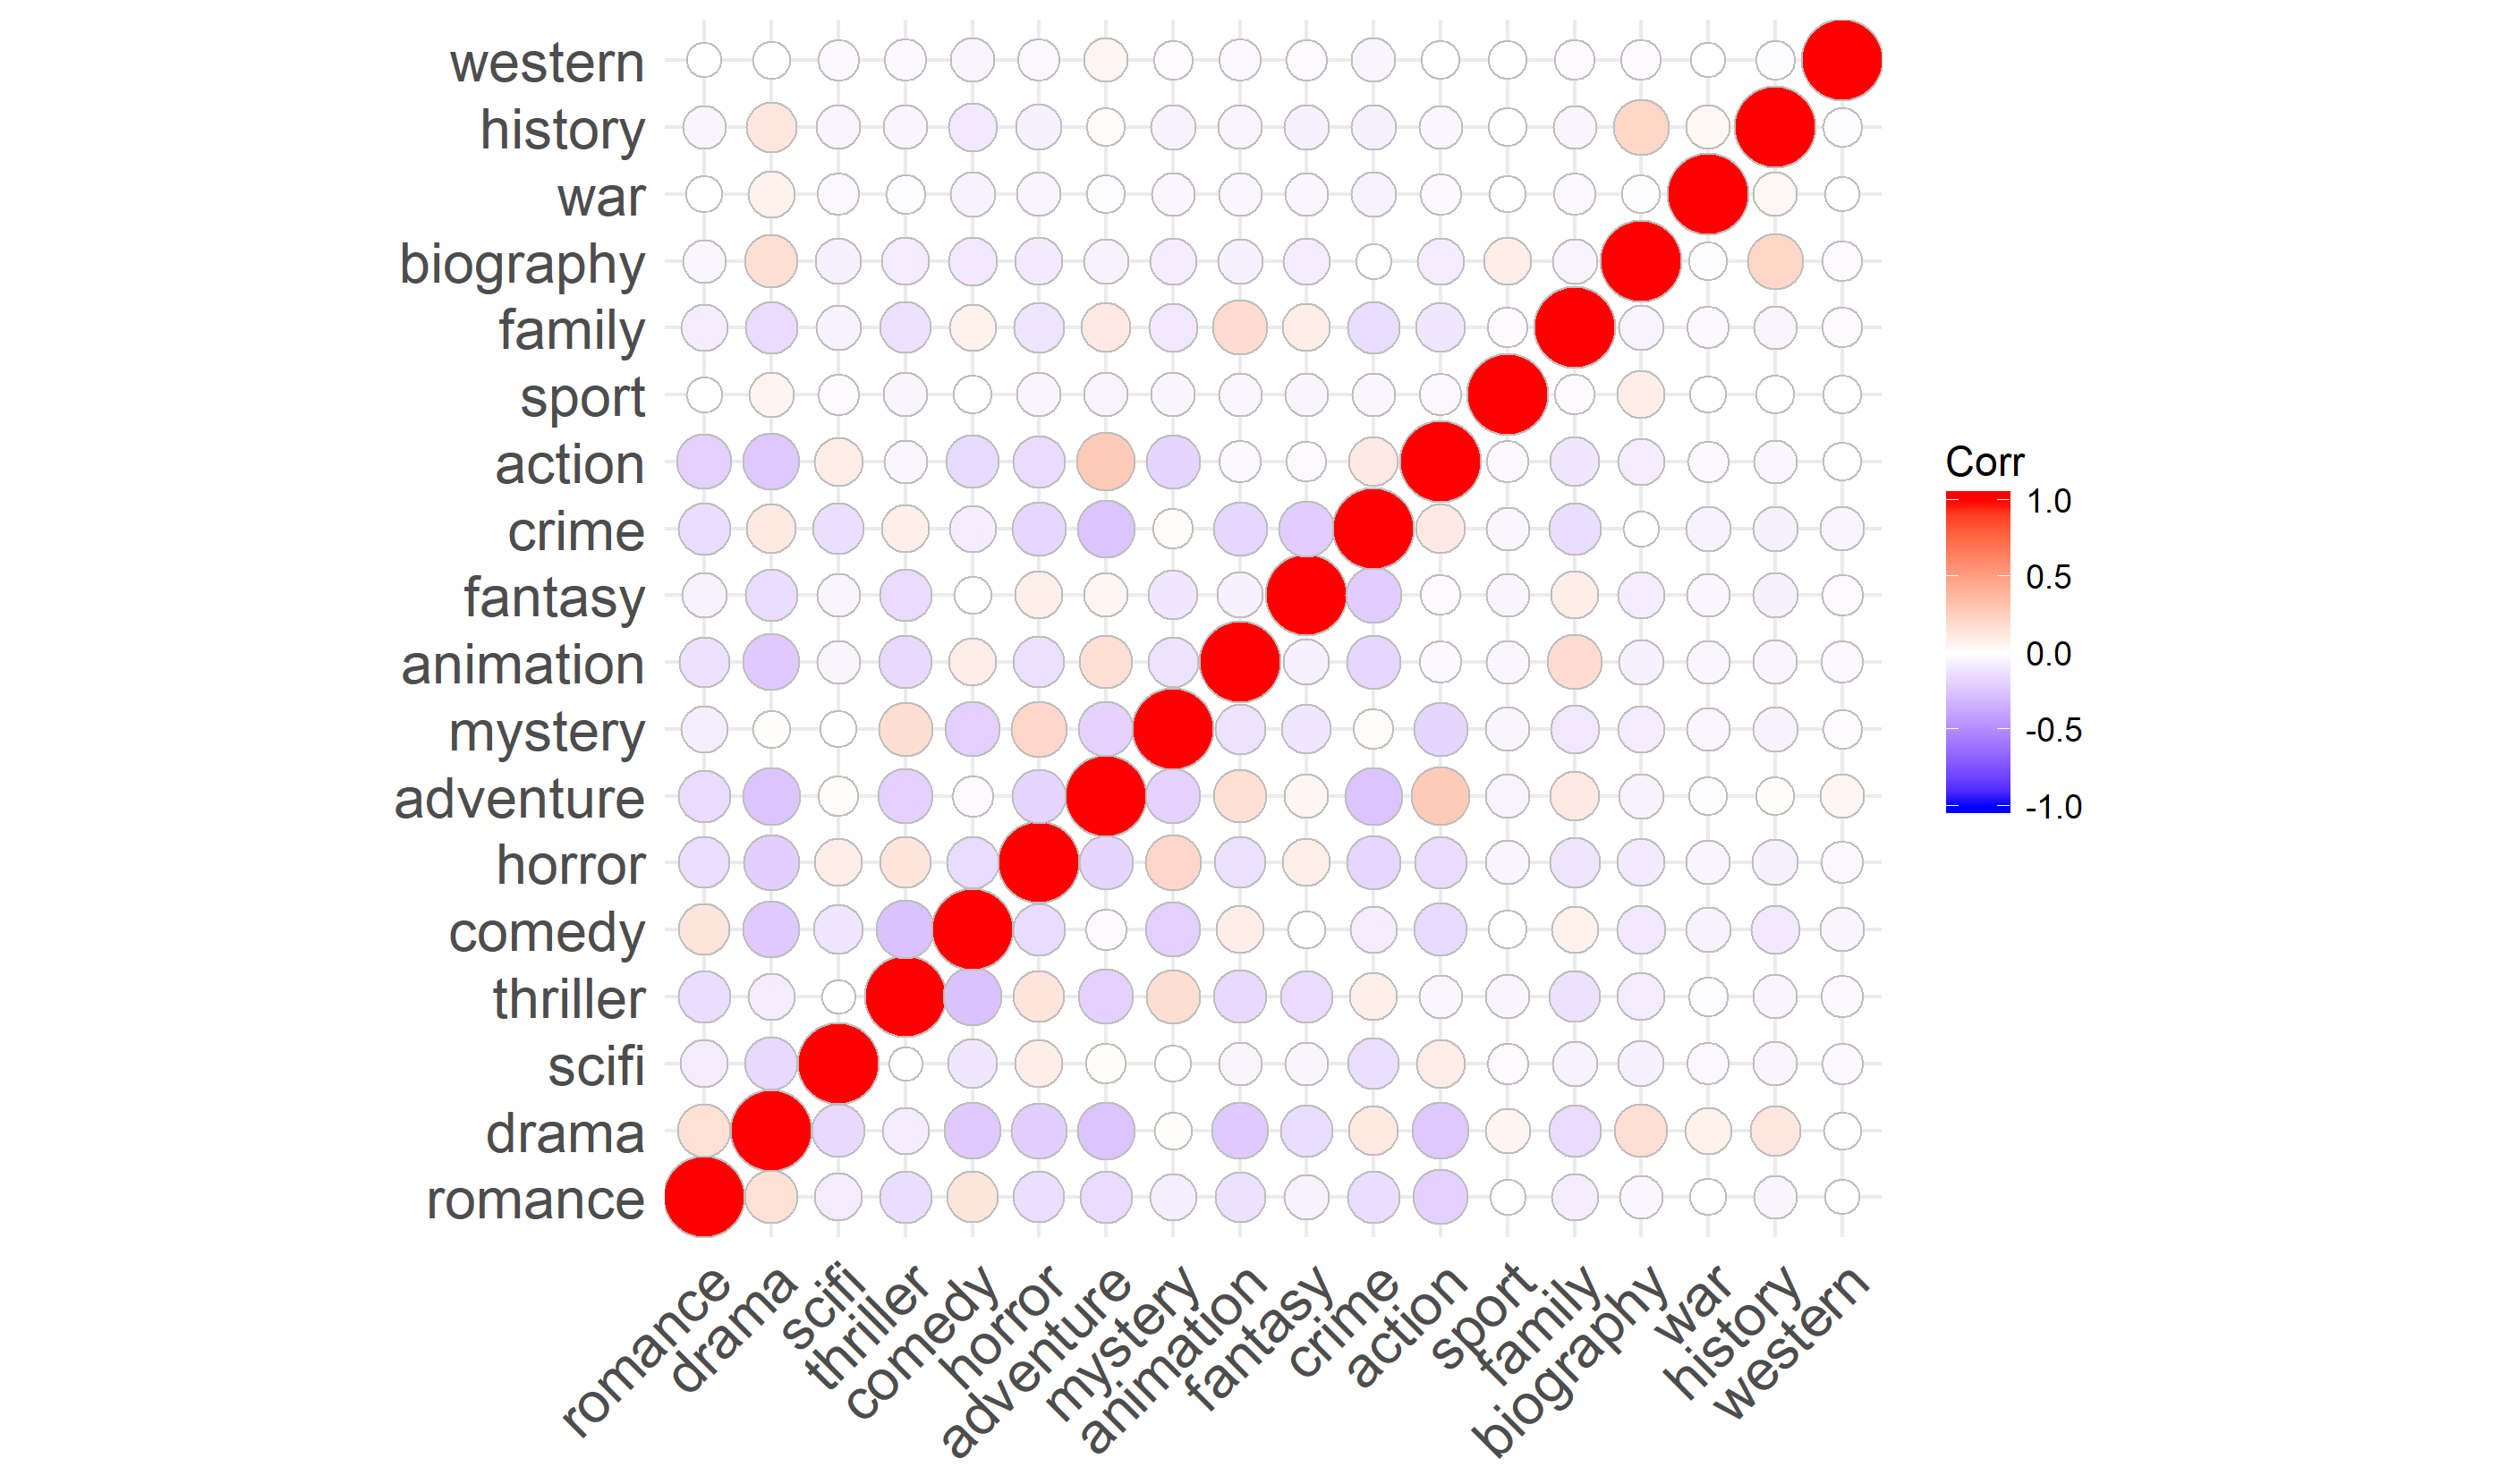
\includegraphics[width=1\textwidth]{correlation.png}
\label{fig:corr}
\end{figure}


As a real example, consider the movie Fight Club. It only has drama assigned as a category on IMDb. Therefore, based on only the first criterion it is equally close to Lion King,  The Lord of the Rings and Se7en (as these all have drama as one of the categories). However, when we add the second criterion, Fight Club has a similarity score of 3 with Se7en (shared genres: drama, crime, mystery), and 1 with Lion King and The Lord of the Rings (the only shared category is drama), respectively. Finally, to introduce higher variation in the movie similarity scores, each movie pair was given an additional point if they were retrieved as part of the same genre category from the IMDb website.

At this point we knew the semantic distance and the genre similarity score between each movie pair, and the next step was to construct the target-decoy and target-competitor pairs. We used our LSA- and genre-similarity scores to select pairs of movies that are likely to be perceived as different and similar as target-competitor and target-decoy pairs, respectively. We considered movie pair A and B as a target-competitor candidate if 1) the two movies fell in the upper 40\% in each others' semantic distance distribution (where a higher distance means the movies are less similar) and 2) their respective genre similarity scores were in the lower 30\% of each others' genre similarity score distribution (where a lower genre similarity score means they are less similar).

 Considering the variety of the movies people encounter, we would naturally expect to find fewer similar movies than dissimilar ones. Based on this assumption, we used a more stringent criteria to find target-decoy pairs: the two movies had to fall 1) in the lower 20\% of each others' semantic distance distribution and 2) in the upper 15\% of each others' genre similarity score distribution. These cut-off values were chosen to provide us with a sufficient number of reasonable matches (601 unique target-decoy and 1,393 target-competitor pairs).
 
 
To increase the power of our test, our aim was to create "quadruplets" of movies: two targets A and B, and their decoys A' and B' (as shown on Figure \ref{fig:diag}). A quadruplet can be used to make two triplets: A, B, A' and A, B, B'. That is, each quadruplet consists one target-competitor and two target-decoy pairs. Using our target-decoy and target-competitor pairs, we created 21,886 unique quadruplets. We classified these quadruplets based on the "quality" of their two target-decoy pairs. We called a target-decoy pair a strict match if they fell within 1) the lower 7.5\% of each others' semantic distance distribution and 2) within the upper 15\% of each others' genre similarity score distribution (these are half the cut-off values we used for creating the target-decoy pairs). 


 We conjectured that the perceived similarity of the target-decoy pairs will be the most problematic part of recreating an attraction effect (as opposed to finding target-competitor pairs that are perceived as different). This is because we have a highly varied stimuli set with a vast number of storyline-genre combinations, which makes it much harder to find two movies that can be considered similar (especially after eliminating sequels). For this reason, a quadruplet was classified as a high-quality quadruplet if both of the target-decoy pairs in it were classified as strict matches.


\cleardoublepage
\newgeometry{left=2cm,bottom=2cm}
\setcounter{savepage}{\arabic{page}}
\begin{landscape}
\pagenumbering{gobble}
\begin{figure}
\caption{Quadruplet selection criteria in Experiment 1.}
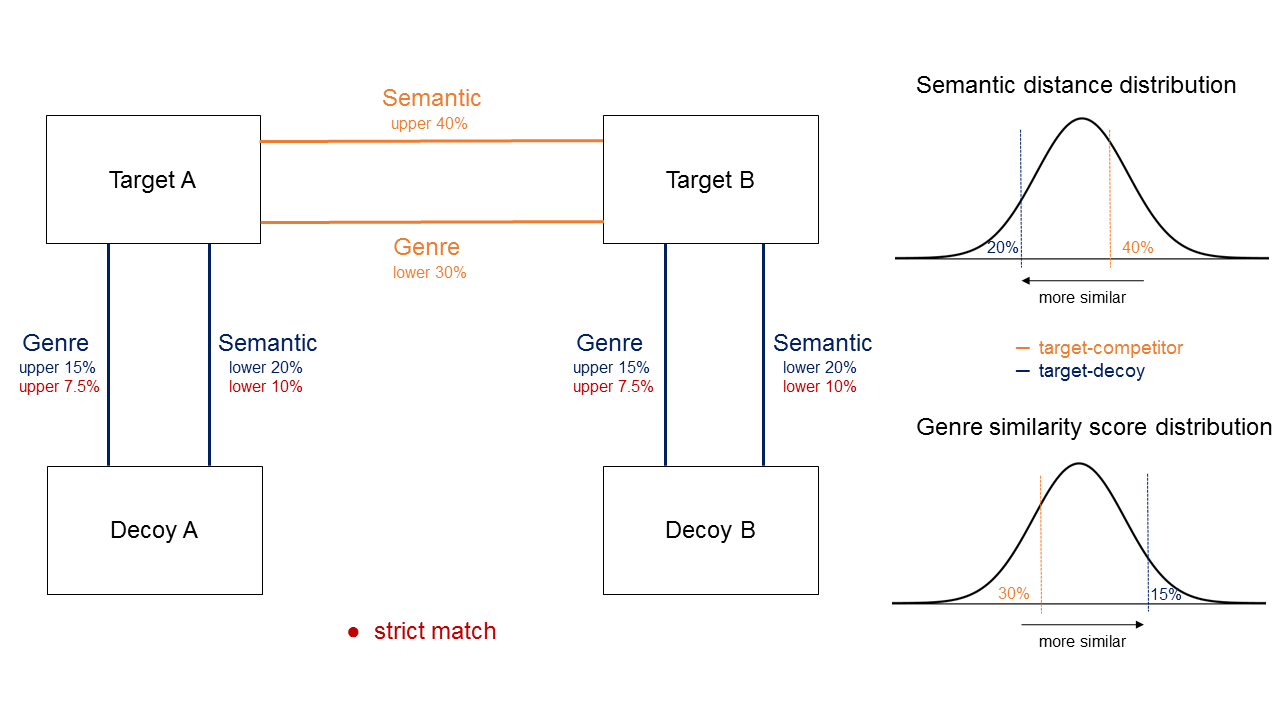
\includegraphics[width=1.45\textwidth]{diagram.png}
\label{fig:diag}
\end{figure}
\end{landscape}
\cleardoublepage
\pagenumbering{arabic}
\setcounter{page}{\thesavepage}
\restoregeometry
 






\subsubsection{Experimental procedure}  \label{experiment_proced}


The experiment consisted of three stages: preference ratings stage, choice stage, and a similarity ratings stage. In the preference ratings stage, we asked for participants' subjective evaluations over the 200 movies ("How do you personally rate this movie?") on a scale from 1 (worst) to 7 (best). We also asked whether the participant had seen the movie before. The 200 movies were presented in a random order for each participant. The ratings stage took about 15-20 minutes on average. The left panel on Figure \ref{fig:exp1_screenshot} shows an example of the ratings task.

Before the choice stage, we created choice triplets for each participant using the ratings they gave in the preference ratings stage in the following way. First, based on the individual ratings from each participant, we identified the subset of quadruplets where: (a) the target and competitor were both rated 4,5,6 or 7, and (b) the two decoy movies were rated at least 3 points lower than the two decoy candidates. Note that we did not require the two decoys in the quadruplet to have the same rating as it would have severely limited the number of quadruplets we could use (e.g., we allowed for quadruplets with ratings 7,7 for the two targets and 4,1 for the two decoys), but we controlled for this difference in our analysis.  

 We then selected the subset of quadruplets where all of the movies had been seen or none of the movies had been seen, to make sure that choice behaviour will not be governed by differences in familiarity with the movies. The result was a bespoke subset of quadruplets for each participant where the target/competitor movies had the same rating and the decoy movies were rated worse. 
 
 However, we did not want the same movie to appear twice as a target/competitor for one participant, and for this reason we used a sequential elminiation techinque: we first chose the quadruplet with the highest combined target-decoy similarity rating, then eliminated all quadruplets with the same target/competitor movies. We repeated these steps until we had a set a of quadruplets with unique target/competitor movies.  

   \cleardoublepage
\newgeometry{left=1cm,bottom=1cm}
\setcounter{savepage}{\arabic{page}}
\begin{landscape}
\pagenumbering{gobble}
\begin{figure}
\caption{Experiment 1 stages: ratings, choice, similarity ratings.}
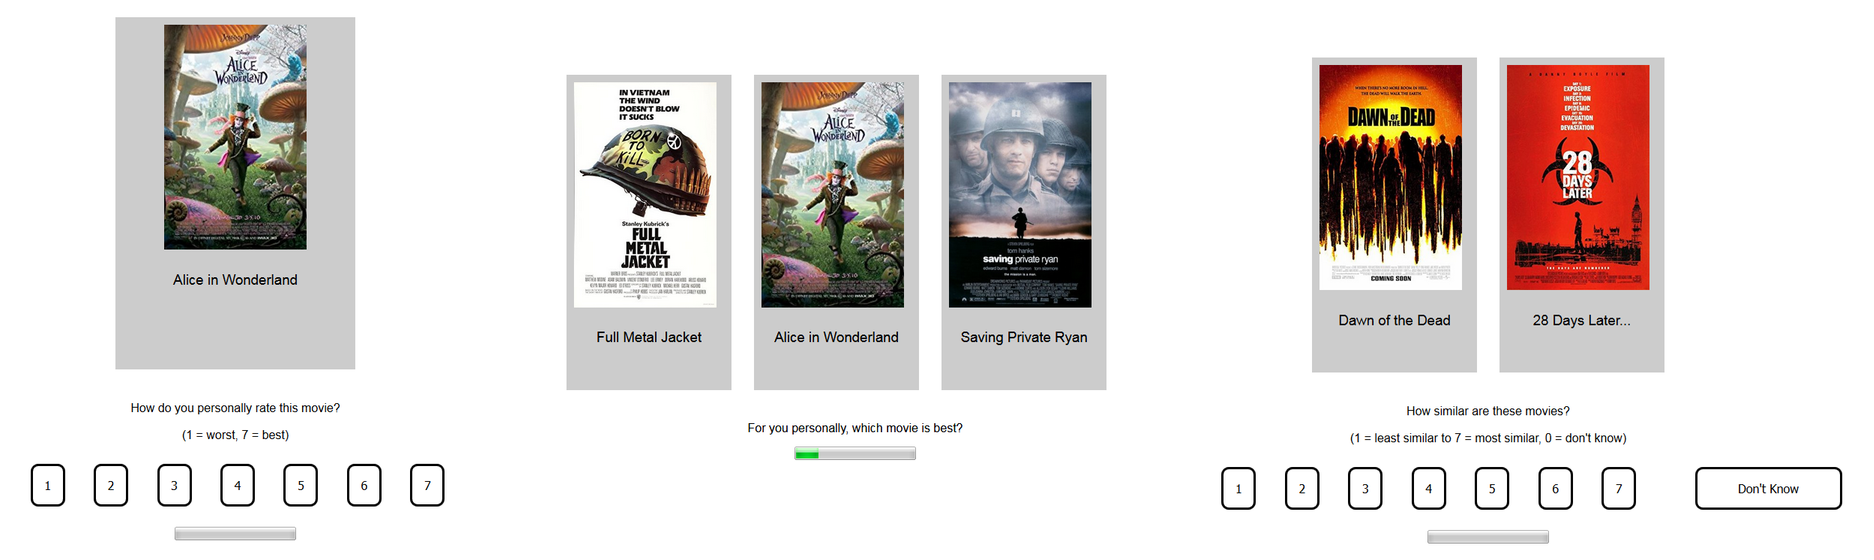
\includegraphics[width=1.7\textwidth]{experipics.png}
\label{fig:exp1_screenshot}
\end{figure}
\end{landscape}
\cleardoublepage
\pagenumbering{arabic}
\setcounter{page}{\thesavepage}
\restoregeometry

 
  We then only invited those participants back for whom we could create at least three high-quality quadruplets this way (corresponding to at least six attraction effect choice triplets where the target-decoy pairs are strict matches). In the choice stage, people were presented with the selected movie triplets in a random order and were asked to choose the one they preferred the most out of the three (see the middle panel on Figure \ref{fig:exp1_screenshot}). 


Because we had to invite people back for the choice stage, we collected data in batches of 50 until we had choice data for at least a 100 participants (after all the exclusion criteria had been applied, see section \ref{exclusion_ref}). 

 
 After the choice stage, those participants whose unique quadruplets included non high-quality quadruplets took part in a third, similarity ratings stage. In this stage, they were asked to rate the similarity of the non-strict match movie pairs on a scale from 1 (least similar) to 7 (most similar), where a "don't know" option was also included. The right panel on Figure \ref{fig:exp1_screenshot} shows an example of the similarity ratings task. Information collected in this similarity rating stage was important to ensure the validity of the test.
 
 Overall 322 participants were recruited from the Prolific Academic subject pool whose first language was English and were paid at an hourly rate of £8. We obtained ethics approval from The University of Warwick's Humanities and Social Sciences Research Ethics Committee (reference number: 50/17-18). The description of the experiment asked for participants who were familiar with American movies. We have not collected data on gender, age and ethnicity, as we did not plan to use this information. The typical Prolific Academic user is from the UK, US or Canada (~ 80\%), below the age of 40 ($\sim$ 75\%), Caucasian ($\sim$ 79\%), female ($\sim$ 60\%) and is in full- or part-time employment ($\sim$ 67\%). Participants who were invited back after the ratings stage were sent an invitation for the choice and similarity ratings stage typically three days after they completed the ratings stage, and were paid after all they completed all three stages.

Out of the 322 participants who completed the rating stage, we could create at least one quadruplet that included movies that had either been all seen or not seen for 262 participants, and for 122 of these participants we could create at least 3 high-quality quadruplets. Out of the 122 participants who were invited back, 114 took part in the choice stage of the experiment.  
 

 
 


\subsubsection{Exclusion criteria} \label{exclusion_ref}

To conduct a rigorous test of the attraction effect, it is crucial that people take the task seriously and reveal their true preferences. Given that individually rating 200 movies can seem somewhat mundane, we specified a set of exclusion criteria to filter those people out who did not take the rating task sufficiently seriously. These were the following. 

We excluded people who fell into the fastest 5\% of the reaction time distribution, the lowest 5\% of the entropy distribution and the upper and lower 5\% of the autocorrelation distribution. Entropy refers to the diversity of the ratings, while autocorrelation takes into account the temporal pattern and measures the extent to which a response depends on previous responses. Thus, this measure aimed to filter out response patterns where people 1) spent an unusually short time completing the task or 2) did not use the whole of the ratings scale or 3) often gave the same ratings for consecutive movies or 4) were giving ratings randomly.

This exclusion criteria was validated by a pilot study, where we collected repeated participant ratings for a set of books and found that the subset of participants with a low correlation between repeated ratings (r $<$ 0.8) were almost exclusively the ones who were also filtered out by these three criteria. After we applied these exclusion criteria to our sample of 114 people, we had choice data from 101 participants.

The study design, exclusion criteria and all the analyses were planned and registered before we collected any choice data. The pre-registration can be accessed at \textcolor{red}{aspred url}. 


\subsection{Results}

Figure \ref{fig:exp1_hist} shows the distribution of the proportion of participants over the number of choice trials, which, by construction, was always even (since one quadruplet included two choice triplets). The minimum number of choice trials was 6, and the maximum was 36. As it can be seen, 87\% of people were presented with at least 8 choice trials. The average number of choice trials was 14.

\begin{figure}[htp!]
\captionsetup{justification=centering}
\centering
\caption{Distribution of the proportion of participants by number of choice trials in Experiment 1.}
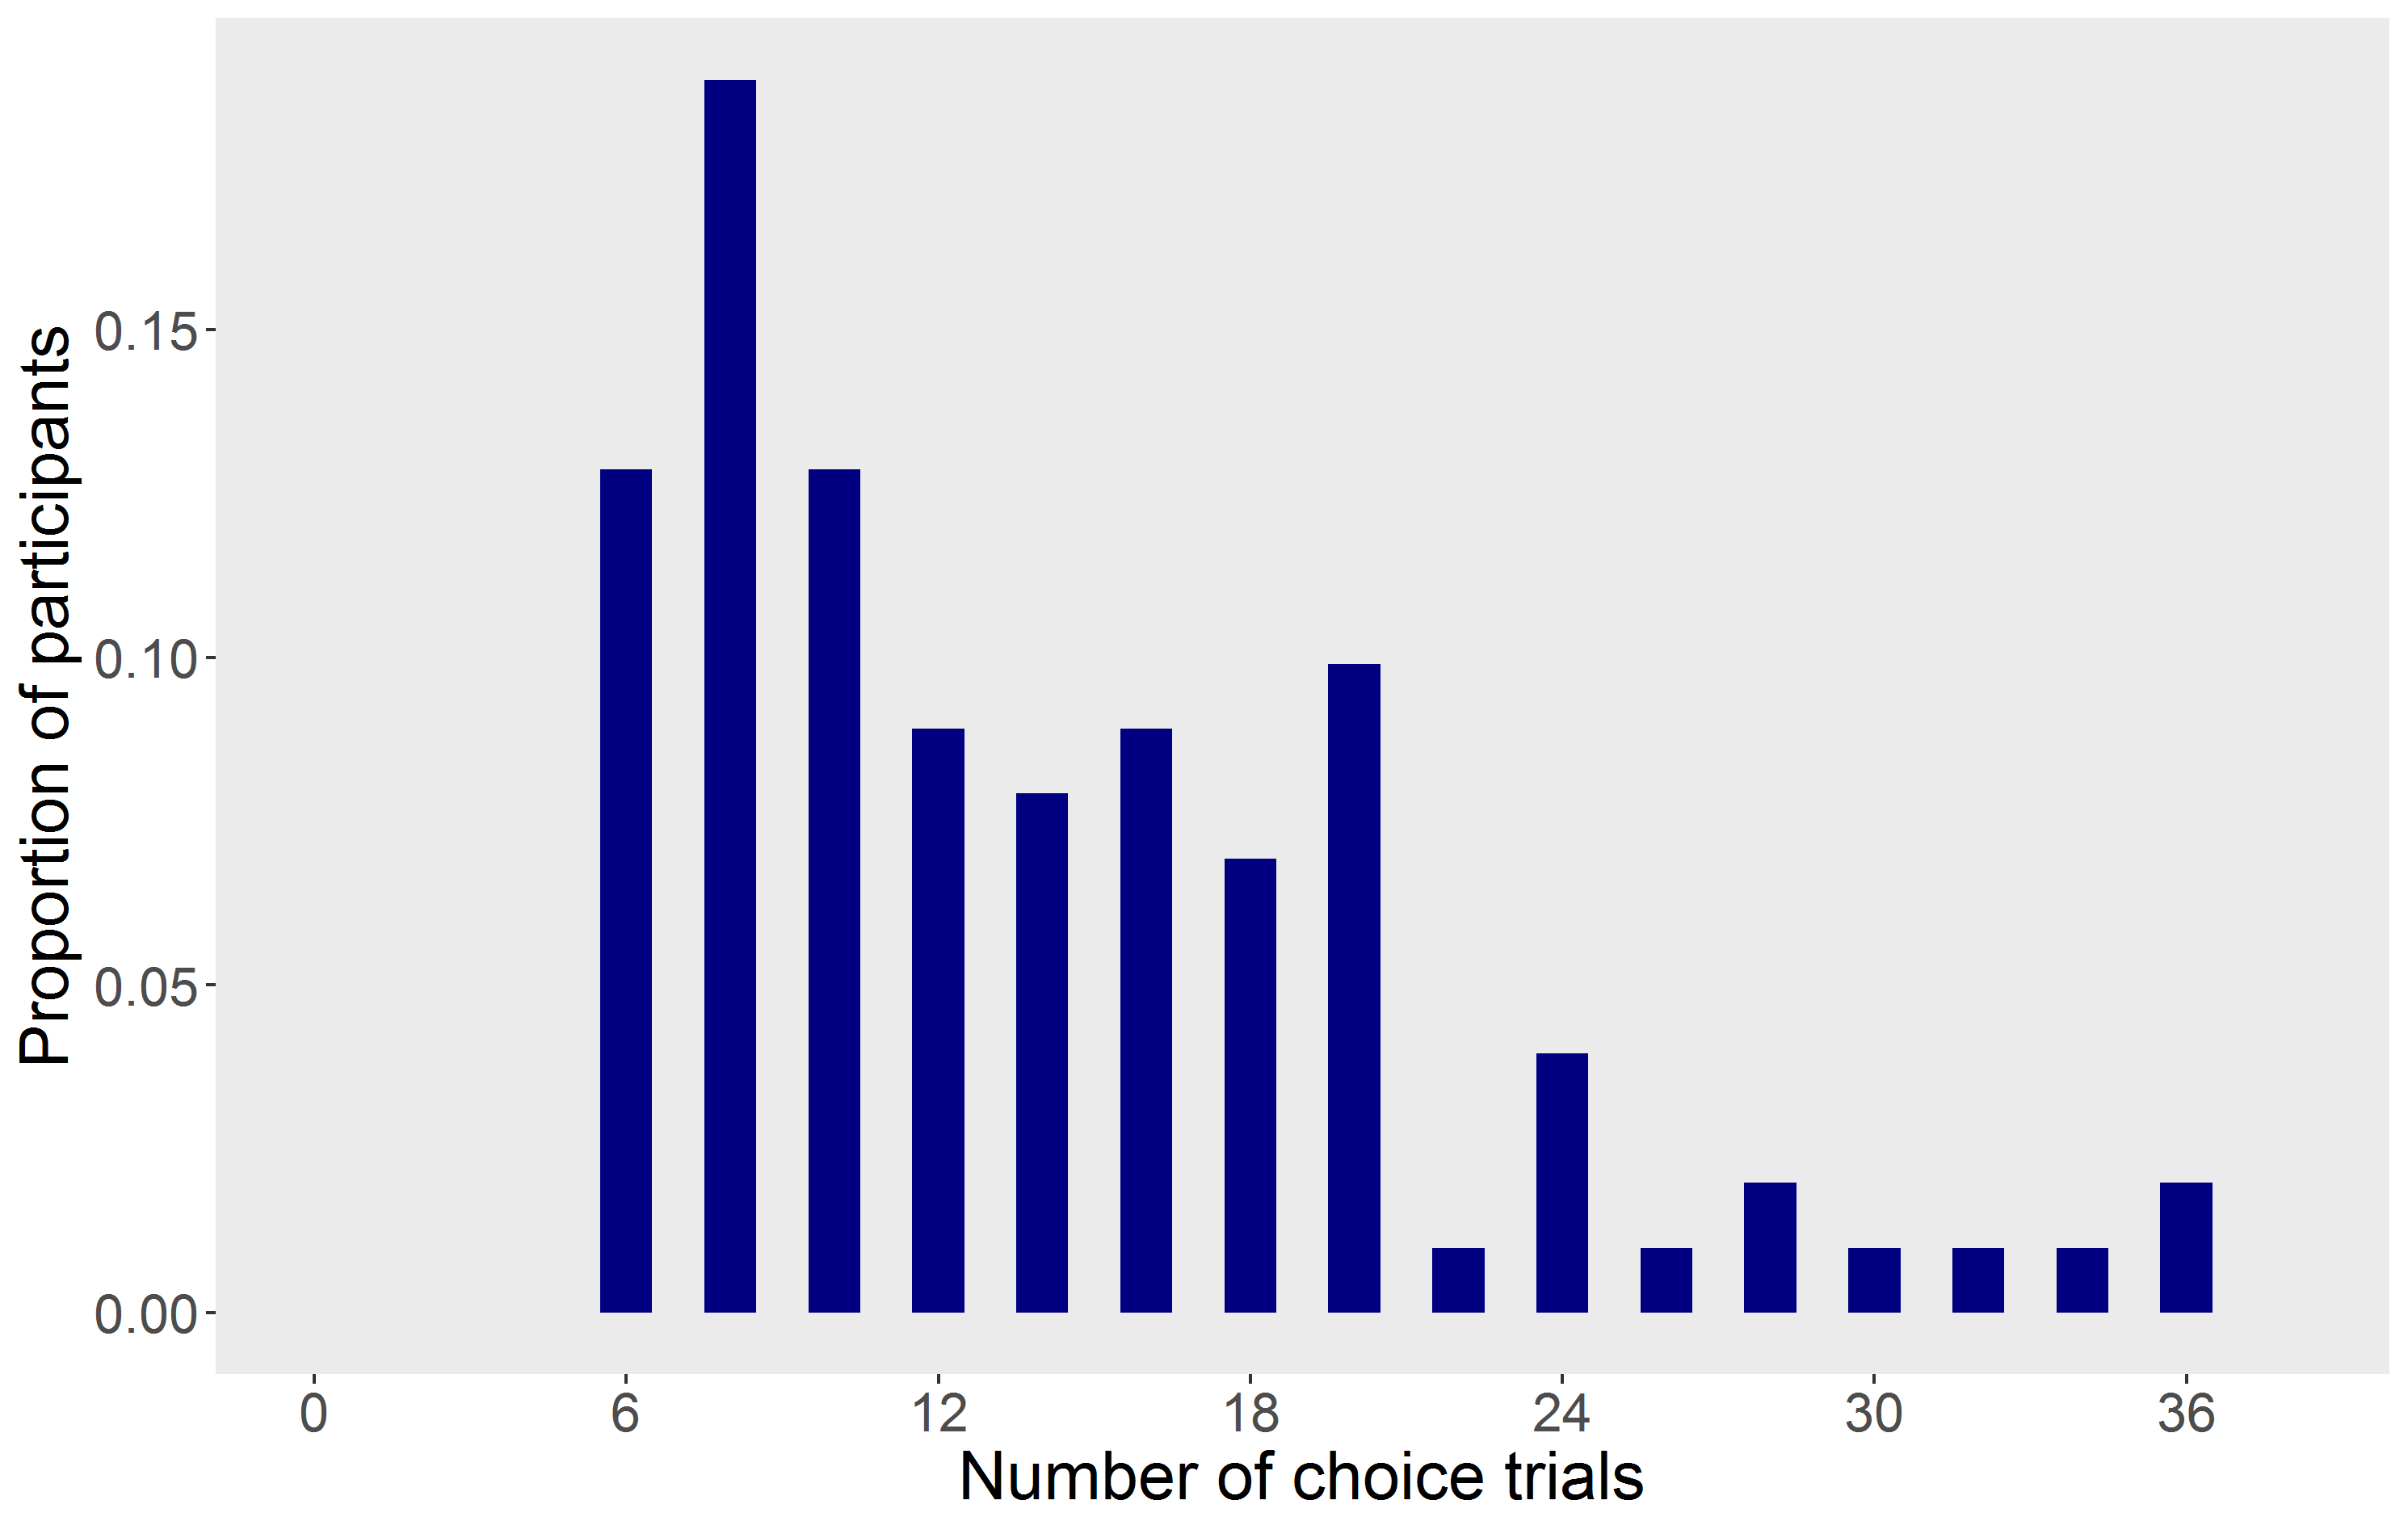
\includegraphics[width=0.8\textwidth]{exp1_hist.png}
\label{fig:exp1_hist}
\end{figure}


As we specified in our pre-registered analysis plan, we excluded any trial in which the participant chose the decoy from the analyses presented below. Figure \ref{fig:exp1_decoytrials} shows that the decoy was rarely chosen, in fact, 61\% of the participants have never chosen it, and less than 4\% people have chosen it in more than 25\% of the trials. This indicates that most people gave reliable ratings in the first stage, and thus were able to identify the dominated decoy in the choice stage.


\begin{figure}
\captionsetup{justification=centering}
\centering
\caption{Distribution of the proportion of participants by proportion of trials where the decoy was chosen in Experiment 1.}
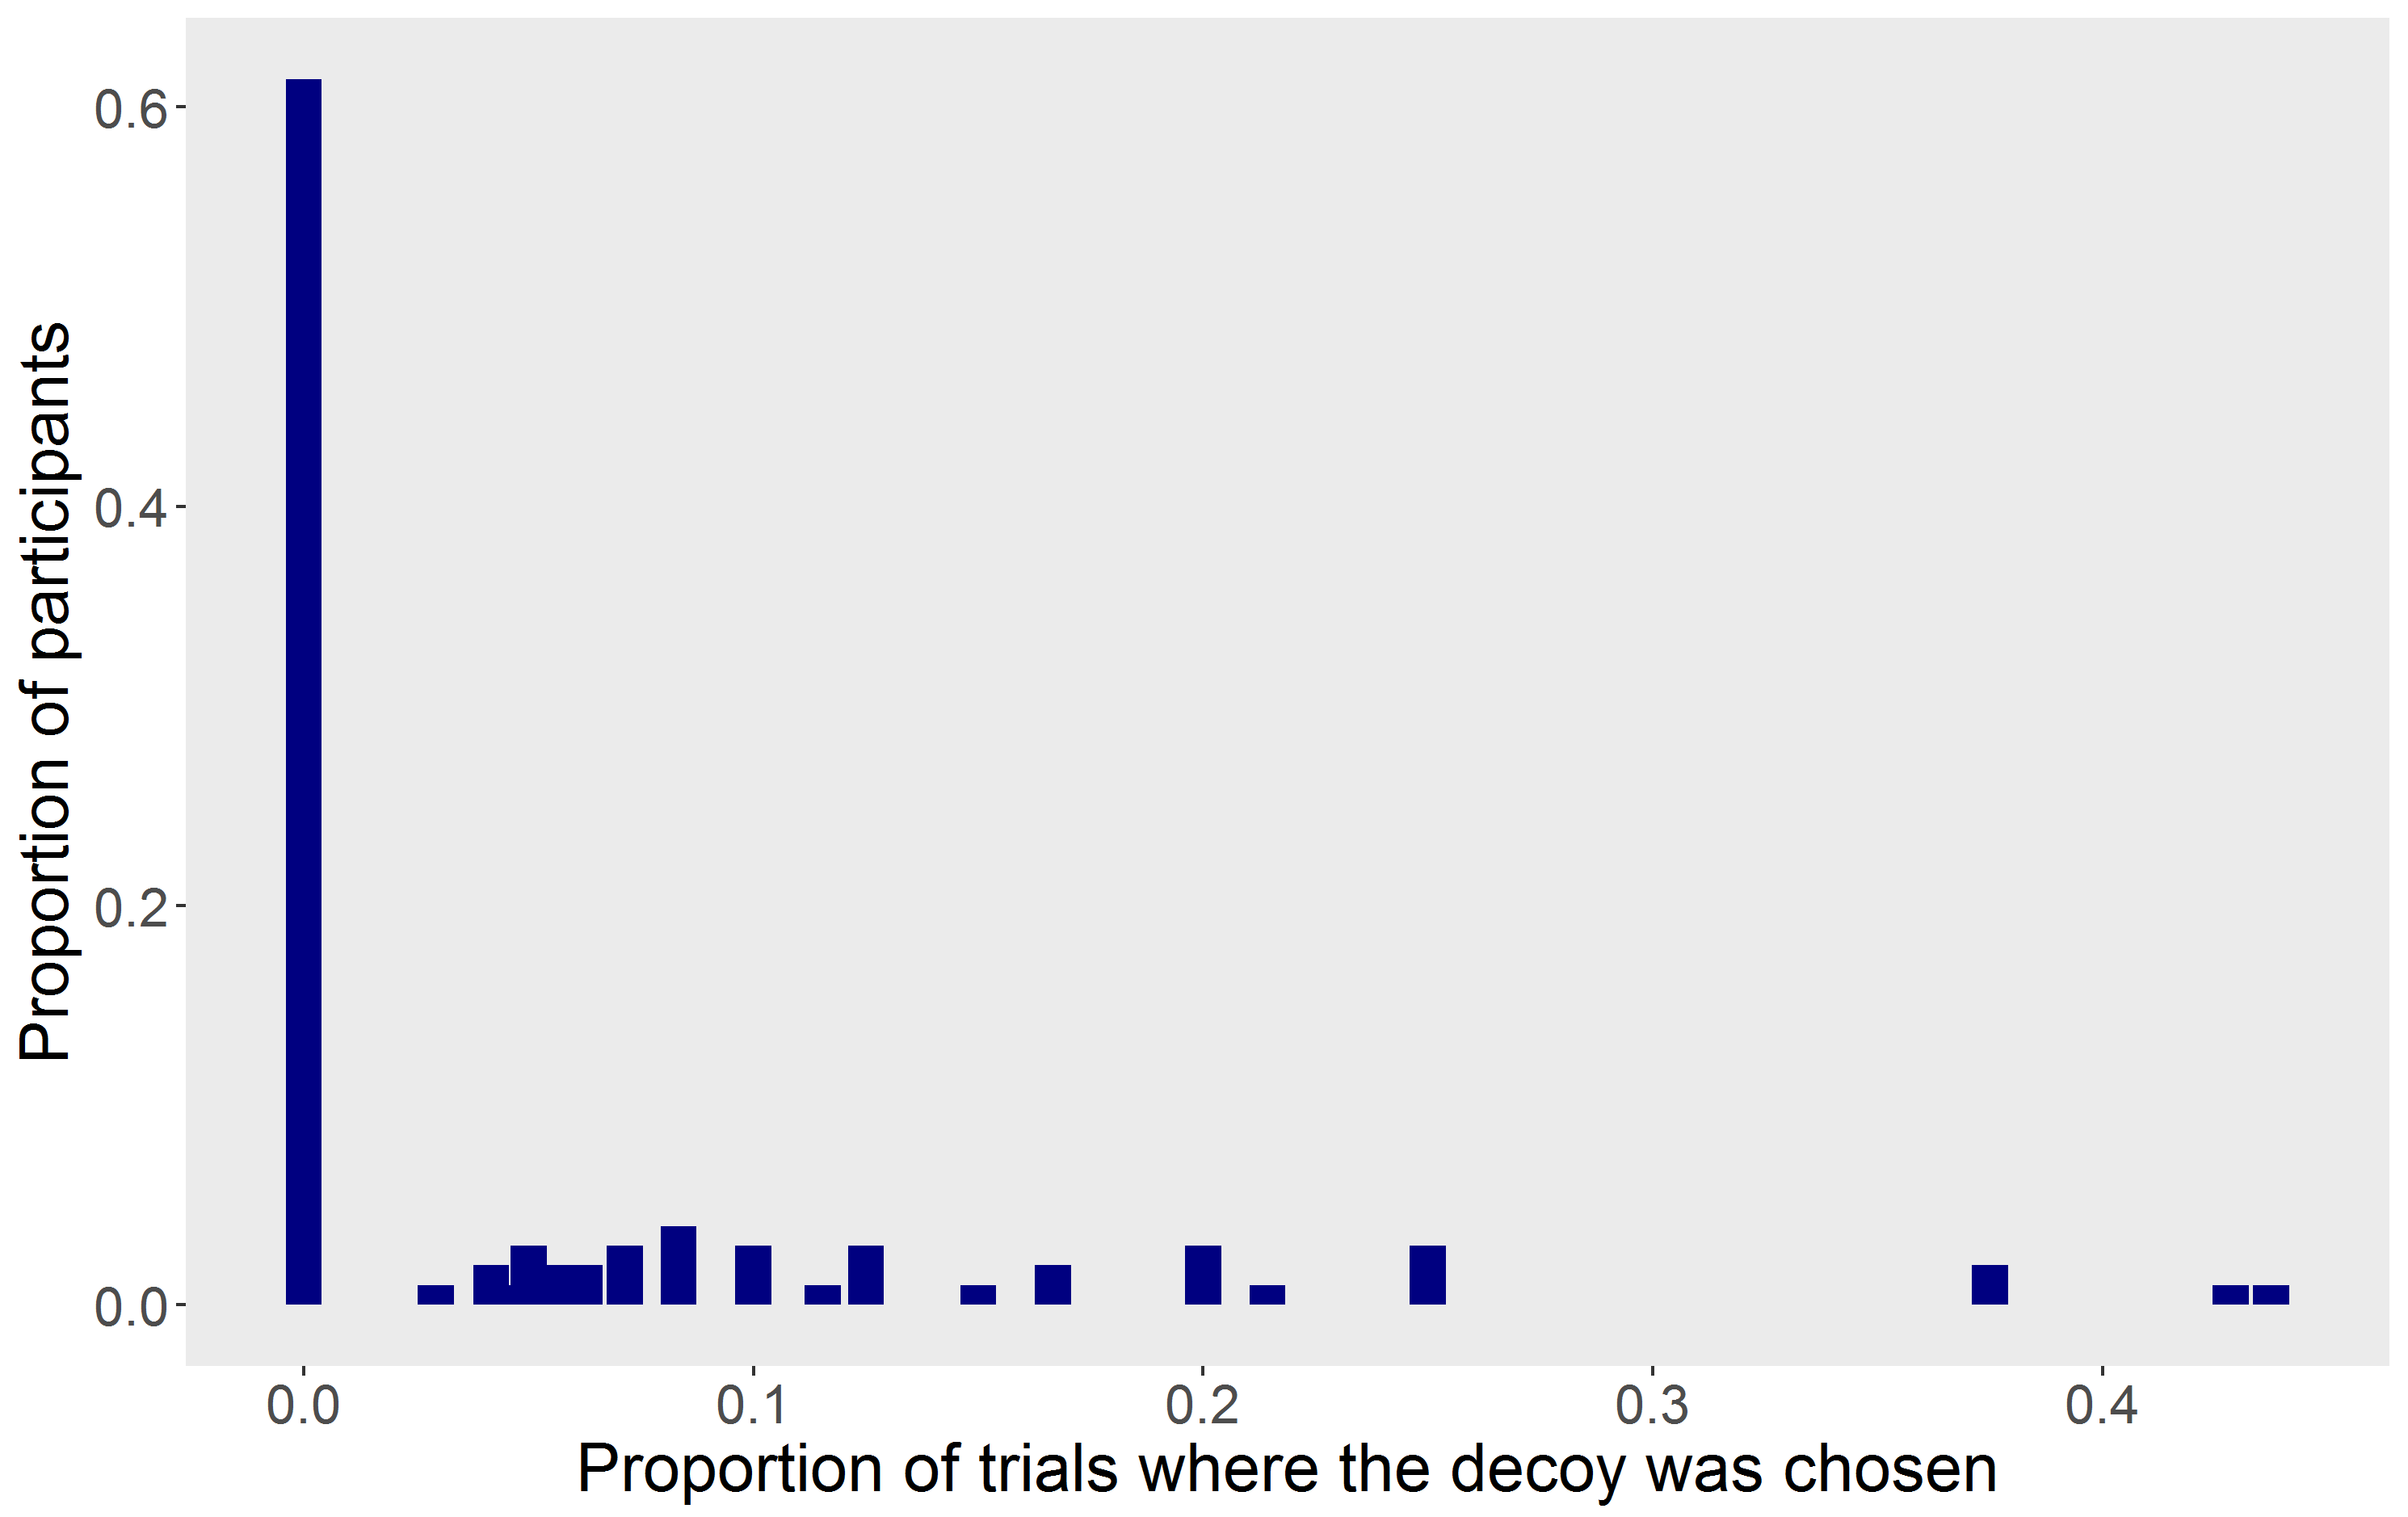
\includegraphics[width=0.8\textwidth]{exp1_decoytrials.png}
\label{fig:exp1_decoytrials}
\end{figure}

%A: We said in the preregistration that we would test if the proportion is above 0.5, which to me sounds like a one sided test? If you don't think it will be a problem, I am happy to report a two-sided one, it does not change the null result anyway. The CIs on Figure 8 did not come from the t-test, they are bootstrapped. Is that okay?

To test for the presence of the attraction effect, we conducted a one-sample t-test to test the hypothesis that the mean of the proportion of trials where the target was chosen  is above 0.5. Therefore, evidence for the alternative hypothesis would indicate an increased likelihood of choosing the target item. 

For this analysis, we used the triplets created from high-quality quadruplets (involving target-decoy pairs that were strict matches). Using a one-sided t-test to test whether participants were more likely to choose the target than the competitor, we found no evidence for the attraction effect (M = 0.5, SD = 0.09), t(100) = 0.39, p = .348. Figure \ref{fig:exp1_t_test} shows the distribution of the proportion of trials where the target was chosen, indicating that the vast majority of participants were indifferent between the target and competitor, meaning that the presence of the decoy did not affect preferences, M = 0.5, 95\% CI [0.49, 0.52].

\begin{figure}[H]
\captionsetup{justification=centering}
\centering
\caption{Distribution of the proportion of trials where the target was chosen in Experiment 1 (triplets with strict target-decoy pairs only). The red dot and error bars show the bootstrapped mean and 95\% CIs.}
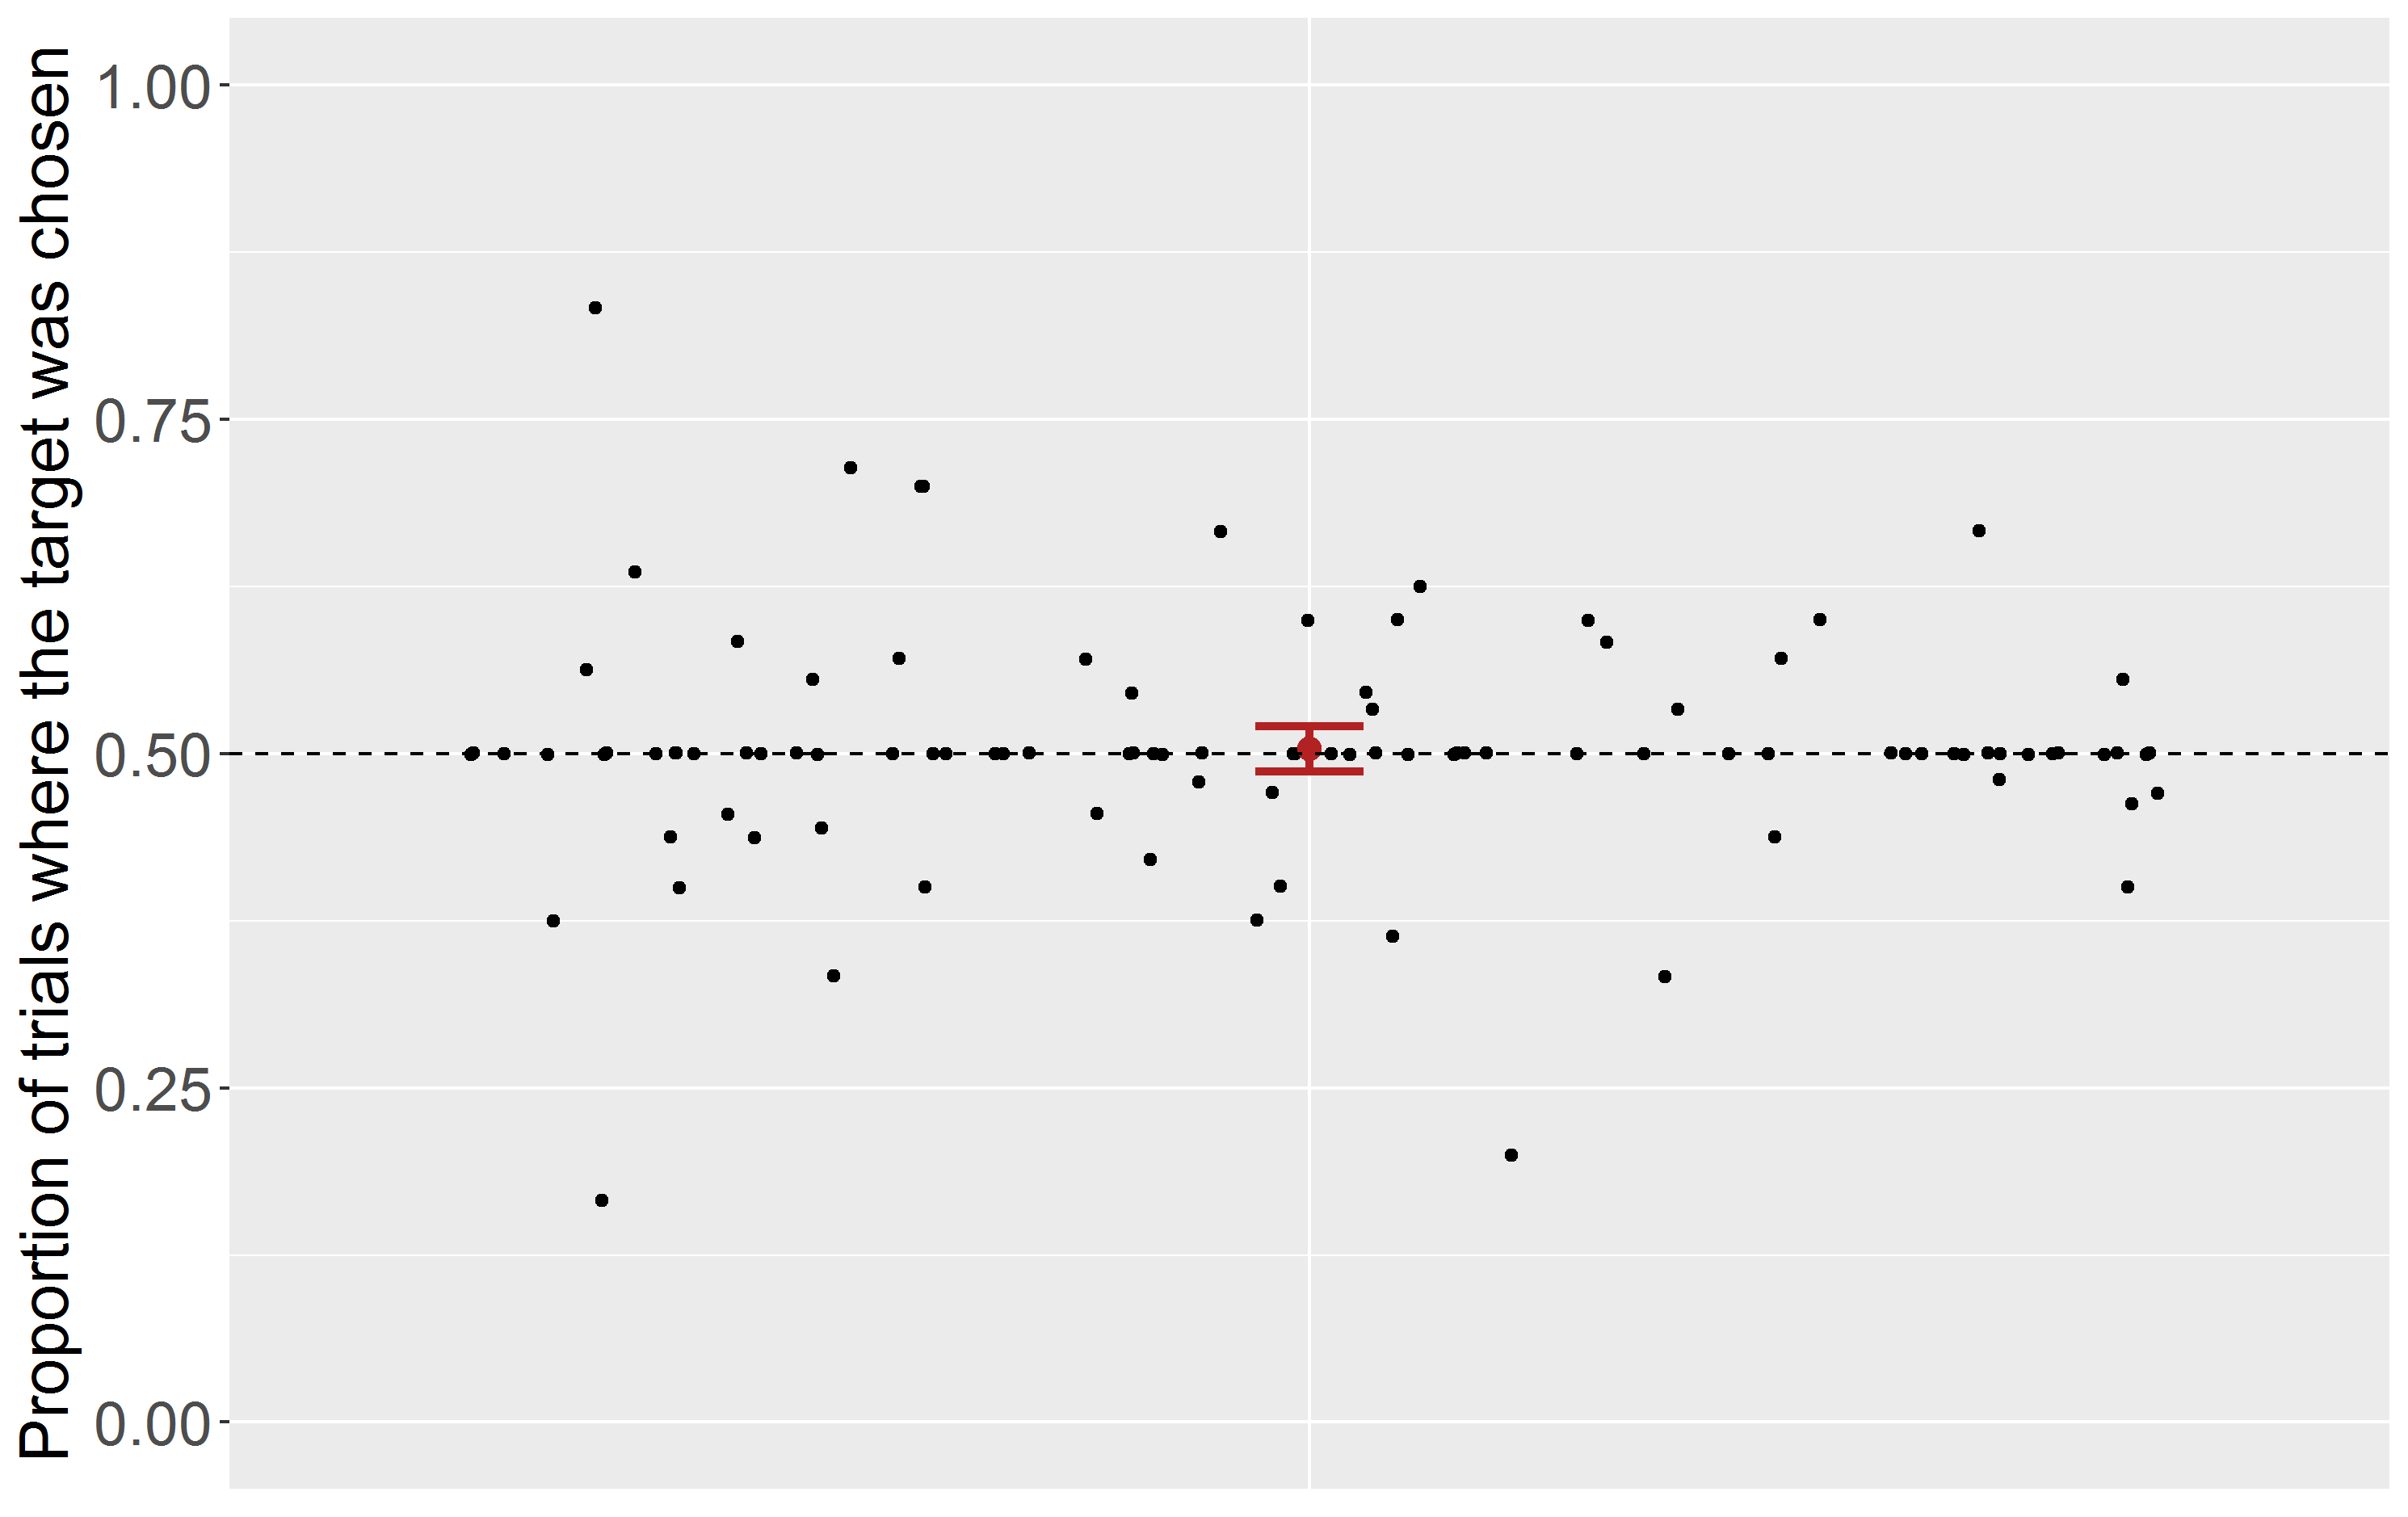
\includegraphics[width=0.75\textwidth]{exp1_highqual.png}
\label{fig:exp1_t_test}
\end{figure}

As specified in our pre-registered plan, we repeated the analysis for triplets with strict target-decoy movie pairs plus triplets created from half the remaining quadruplets with the lowest combined target-decoy semantic distance (we refer to these as the "better half" of the remaining quadruplets), and again found no evidence for the attraction effect (M = 0.51, SD = 0.08), t(100) = 0.28, p = .22 (for the distribution of the proportion of trials where the target was chosen in this subset of data, see Appendix \textcolor{red}{x}). 

 
Our last planned analysis was a mixed effects logistic regression model with subject-specific random intercepts, where for each trial, we predict the likelihood of choosing the target item with the following explanatory variables: having seen all three of the movies (as opposed to not having seen any of them), target-decoy and target-competitor semantic/genre distance, and the target-decoy rating difference (by the design of the triplet construction method, this was at least 3, and at most 6). Table \ref{latentattr_exp1reg} shows the results from this regression.



\begin{table}[!htbp] \centering 
\captionsetup{justification=centering}
  \caption{Odds-ratios and 95\% CIs from a mixed-effects logistic model with subject-specific intercepts, Experiment 1. (T - Target, C - Competitor, D - Decoy)} 
  \label{latentattr_exp1reg} 
\resizebox{9cm}{!}{\begin{tabular}{@{\extracolsep{5pt}}lc} 
\\[-1.8ex]\hline 
\hline \\[-1.8ex] 
 & \multicolumn{1}{c}{\textit{Dependent variable:}} \\ 
\cline{2-2} 
\\[-1.8ex] & Target chosen \\ 
\hline \\[-1.8ex] 
 Seen all & 1.156 (0.844, 1.589) \\ 
  TC semantic distance & 0.980 (0.878, 1.093) \\ 
  TD semantic distance & 1.015 (0.910, 1.131) \\ 
  TC genre distance & 0.993 (0.890, 1.107) \\ 
  TD genre distance & 0.972 (0.872, 1.084) \\ 
  TD rating difference & 0.908 (0.789, 1.046) \\ 
  Intercept & 0.992 (0.628, 1.566) \\ 
 \hline \\[-1.8ex] 
Observations & 1,418 \\ 
Log Likelihood & $-$978.245 \\ 
Akaike Inf. Crit. & 1,972.490 \\ 
Bayesian Inf. Crit. & 2,014.546 \\ 
\hline 
\hline \\[-1.8ex] 
\textit{Note:}  & \multicolumn{1}{r}{$^{*}$p$<$0.1; $^{**}$p$<$0.05; $^{***}$p$<$0.01} \\ 
\end{tabular} } 
\end{table} 

As it can be seen, familiarity with the movies, preference difference between the target and decoy movies, and the semantic/genre distance between the target-decoy and target-competitor pairs do not affect the likelihood that the target will be chosen. Based on this model, we can predict the probability of choosing the target in an "ideal" attraction effect situation, where the target-decoy rating difference is at its maximum (6), all the movies had been seen in the triplet, and the genre/semantic difference between the target-decoy and target-competitor pairs are at their respective minimum and maximum. This predicted proportion\footnote{Based on a logistic regression without mixed effects.} is only 43\%, 95\% CI [30, 57], which further shows the lack of an increased tendency to choose the target even in choice situations where the attraction effect should most likely be observed.


We can only speculate about the underlying reason(s) why we did not see an increased preference for the target in our experiment. One possible explanation for our results is that the attraction effect is simply absent in settings where choice options are complex objects, as argued by \citeA{Frederick2014} and \citeA{Yang2014}. While this is one possible explanation for our results, we cannot be certain unless we can safely claim that our experimental methodology have managed to satisfy all the criteria required for a stringent test of the attraction effect. Testing the attraction effect with naturalistic stimuli is a complex task, as it poses several challenges to the standard experimental methodology commonly used in research focusing on this decision bias. 


First, naturalistic objects differ from numerical stimuli as we cannot infer the relative value of each option "on the spot". To circumvent this issue, we added a ratings stage before the actual choice task, and there was at least a day's difference between the time of the two task. One natural concern could be that this might have reduced the reliability of ratings. However, the results have shown that participants were (1) indifferent between the options they have previously rated the same and (2) rarely ended up choosing the dominated option. These results indicate that people gave honest answers in the ratings stage and their preferences did not change over time. 

Second, one must make sure that people are sufficiently interested in the stimuli. With numerical stimuli, interest can be sustained by an incentive-compatible experimental design. To ensure these criteria are met in our experiment, we used the most popular movies on IMDb, used a very strict exclusion criteria to exclude people who did not take the task seriously, and also controlled for familiarity with the choice options, but this did not modulate the effect.  


Third, the similarity comparison process might differ between options with  numerical and naturalistic attributes. The perceived similarity of the target and decoy is a crucial assumption, as many choice models rely on it to be able to produce the attraction effect (see subsection \ref{AE intro}). To ensure maximal similarity between the target and decoy, we have used all available information on our movies, including storyline, actors, and genres, to create the target-decoy and target-competitor pairs, and conducted separate analyses based on the quality of the match. However, this still does not ensure that participants perceived the target-decoy pairs as similar and the target-competitor pair as different. 



Fortunately, we have collected information on perceived similarity for a small subset of movie pairs that did not qualify as strict matches based on our selection criteria, which allows us to estimate the extent problem. Specifically, we have at least one similarity rating for 184 and 203 unique target-decoy and target-competitor pairs, which constitute 16\% and 18\% of all unique choice triplets, respectively. Figure \ref{fig:exp1_simrat} shows the distribution of the similarity ratings for these target-decoy and target-competitor pairs.



 \begin{figure}[!htb]
 \captionsetup{justification=centering}
\centering
\caption{Distribution target-competitor and target-decoy similarity ratings in Experiment 1.}
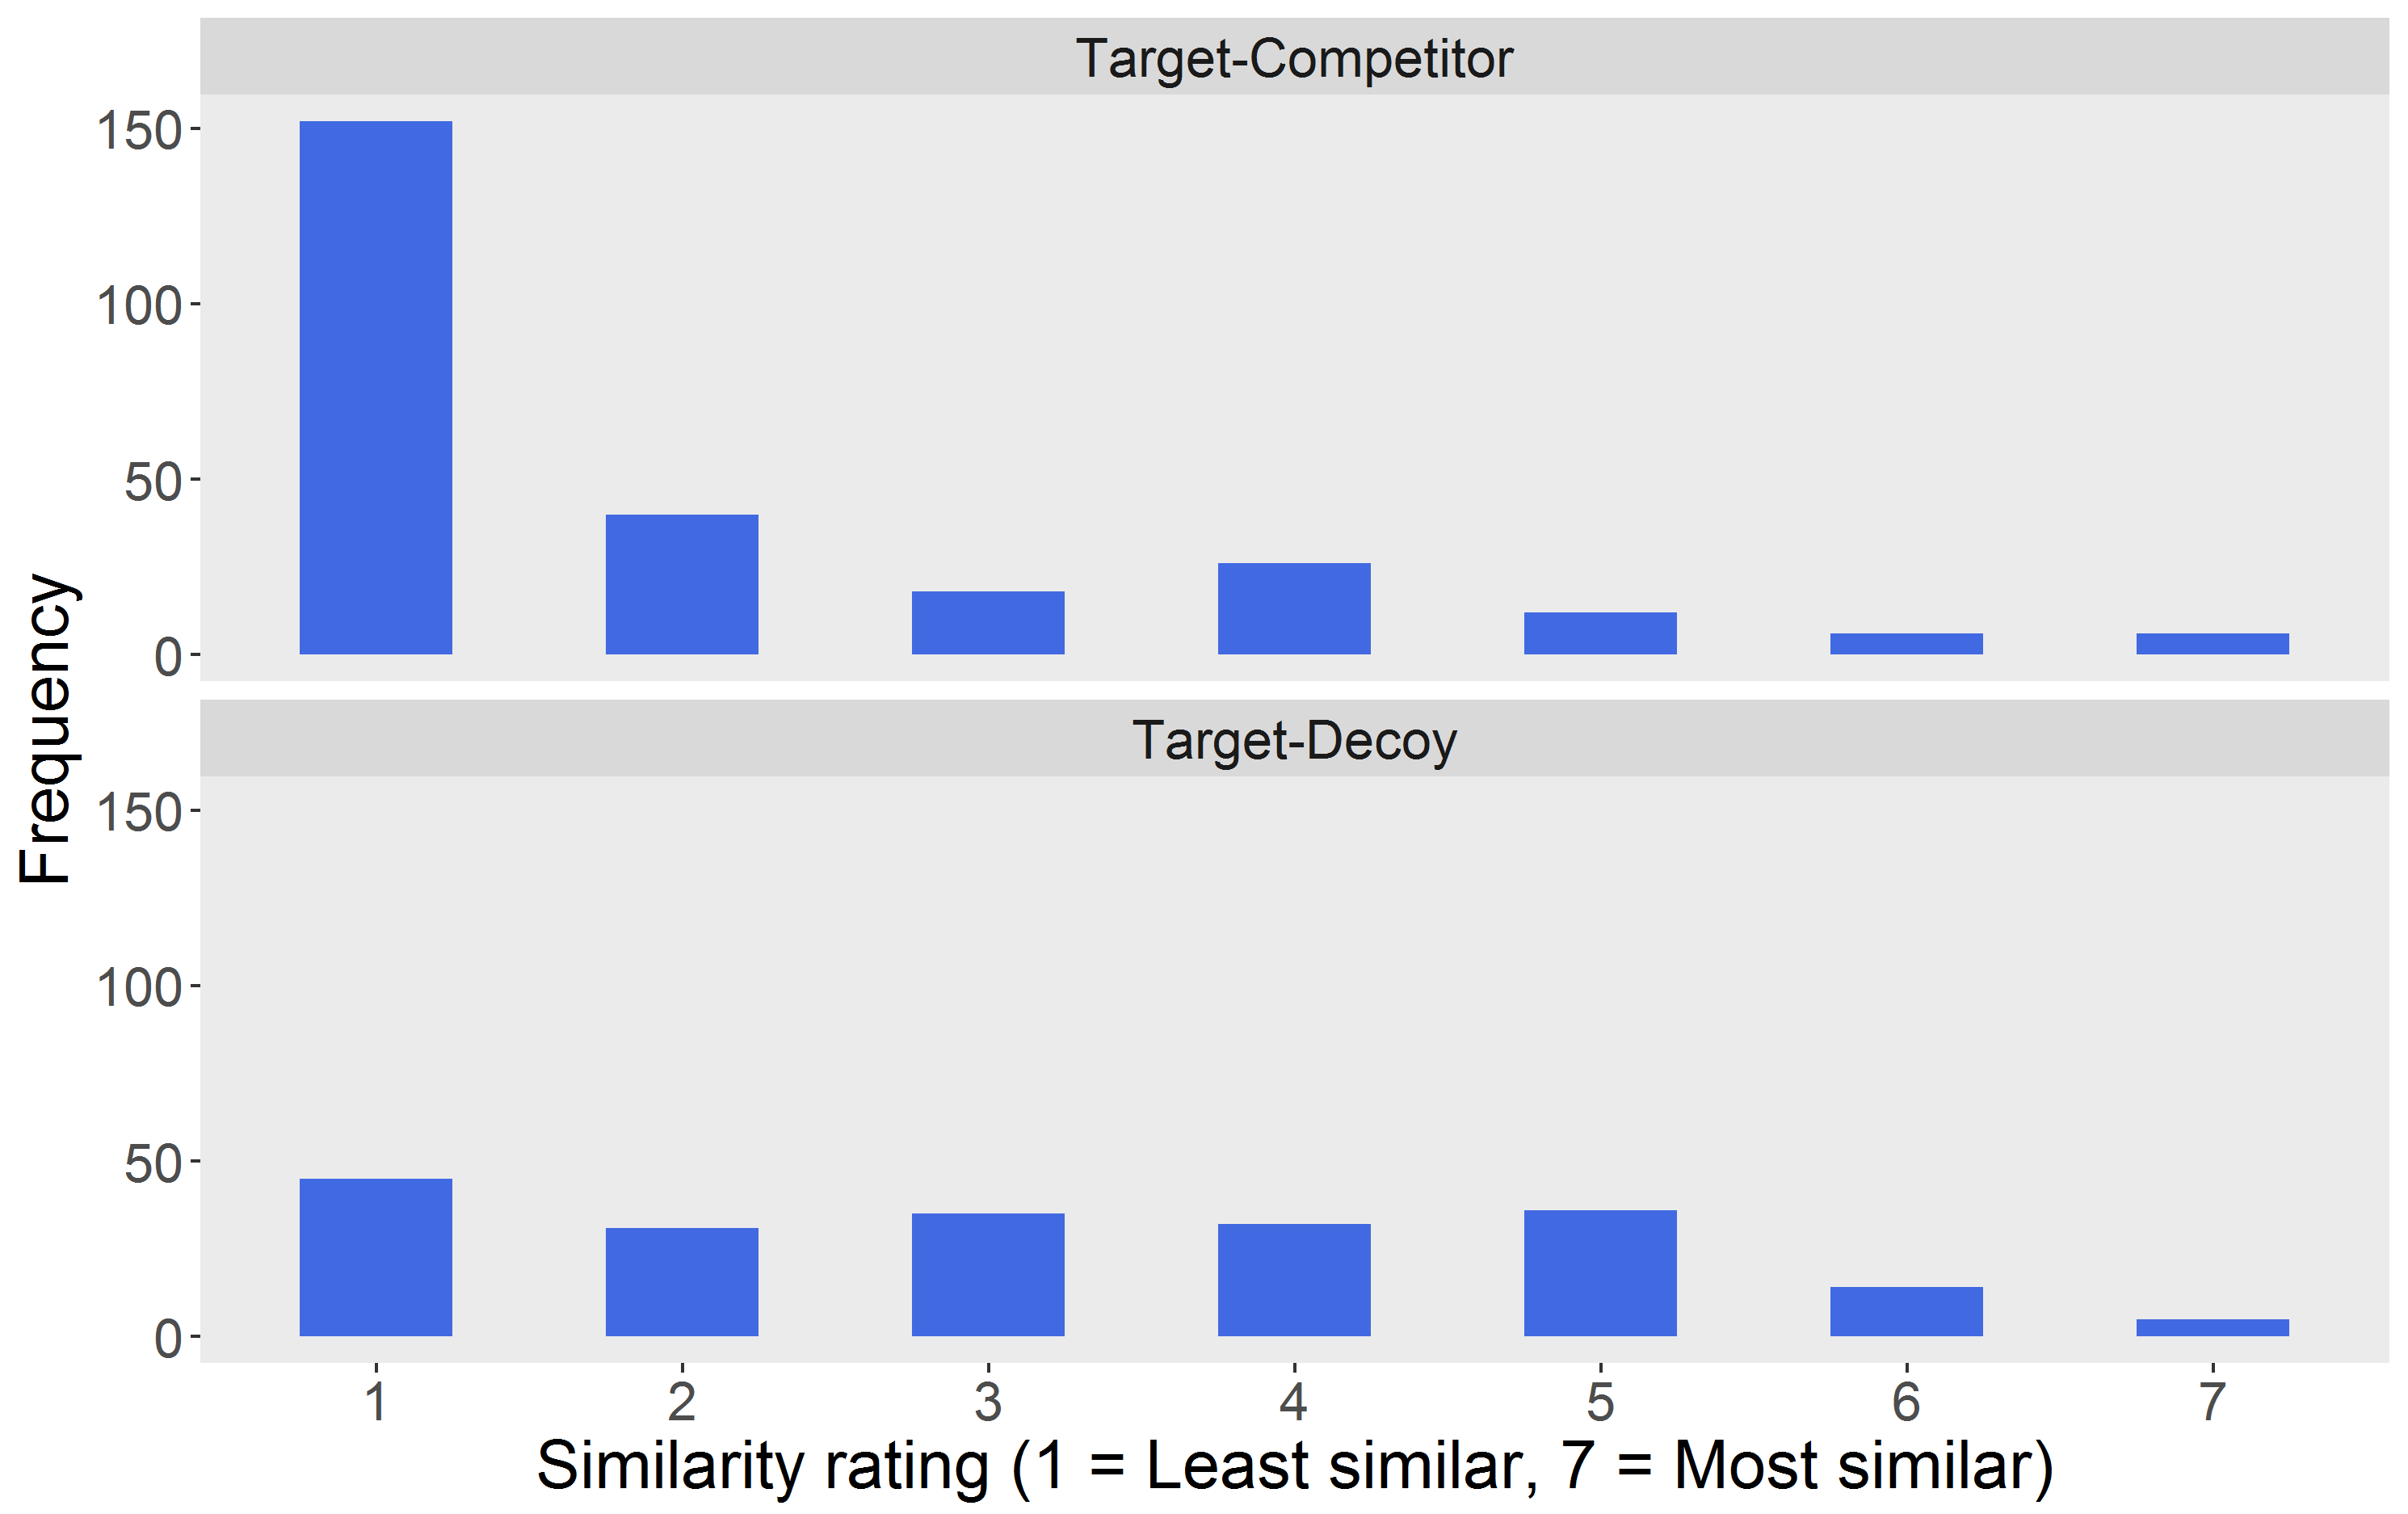
\includegraphics[width=0.8\textwidth]{exp1_similarityratings.png}
\label{fig:exp1_simrat}
\end{figure}

It seems that while most target-competitor movie pairs were given low similarity ratings, showing that they were perceived as markedly different (as we hoped), participants generally did not perceive our target-decoy pairs to be very similar. Although it is worth keeping in mind that we asked for similarity ratings for this subset of movie pairs exactly because we were worried that they might not be perceived as different/similar enough (therefore, it is likely that target-deocy pairs that were strict matches were perceived as more similar than the non-strict matches), but the very low target-decoy similarity ratings still cast doubt on the general efficacy of our triplet selection criteria. 

While we recognised that creating pairs of similar movies is the most challenging part of the experimental design, this lack of perceived similarity is highly problematic when designing a test of the attraction effect. Specifically, if the proximity of the target an decoy are not recognised, then the choice task simplifies to a situation with two, equally good, distinct options, and a third, inferior option. In this case, we would expect that the decoy will almost never be chosen and that the two, equally good options will be chosen equally frequently, which is exactly the pattern we have seen in our results. 


%A: deleted regression with N=20, it's too weak to be convincing and I can speculate without it as well


\subsection{Discussion}

Our aim in Experiment 1 was to replicate the attraction effect using naturalistic, real-world stimuli. Our estimate is that adding a dominated decoy to a binary choice set did not increase preference for the dominating target. We are 95\% confident that the true proportion of trials where the target was chosen is between 49\% and 52\%. In addition, the tendency to choose the target was not affected by participants' familiarity with the movies, the target-decoy rating difference, or the semantic/genre proximity of the target-decoy and target-competitor pairs.

Furthermore, the distribution of the target-decoy similarity ratings from a subset of triplets show that participants rarely perceived the target-decoy pairs as similar. This indicates that (at least) some of the triplets we created did not manage to invoke an attraction effect choice situation.


Why did our stimuli selection method fail to produce movie pairs that are similar? As we mentioned in section \ref{choice_selection}, while the latent semantic solution was successful in retrieving common themes and aspects of each movie's storyline, genre differences are not captured well in this framework (as a certain theme can appear in very different contexts), and it is possible that they are central to the similarity judgement process. 

While our genre matching criteria were supposed to account for this problem, it is possible that matching movies along 18 genre types simply does not capture subtle genre differences that are crucial in judging the similarity between two movies. This problem is further exacerbated by the fact that many movies have only one category assigned on IMDb, making it much harder to establish movie similarity along the genre dimension.

 For example, The Life of Brian has comedy as the only category assigned, whereas Monty Python and The Holy Grail has adventure, comedy and fantasy as genre categories, which means that our algorithm does not identify these two movies as similar enough along the genre dimension despite the fact that they are both Monty Python movies (and would probably be considered as similar by most people).
 
 To summarise, in Experiment 1, we find no attraction effect at all. However, the  low target-decoy similarity ratings suggest that in a significant proportion of the trials, we simply failed to create an attraction effect type situation. To conduct a rigorous test of the attraction effect using the same stimuli, this problem needs to be accounted for.
 
\newpage

\section{Experiment 2} 


Experiment 2 also aimed to test the attraction effect with the same naturalistic choice options, while addressing the problems encountered in Experiment 1. Specifically, to ensure that target-decoy pairs were perceived similar and that target-competitor pairs were perceived as different, we used similarity ratings from a  separate, independent group of participants to help construct choice triplets. We also collected similarity ratings on every target-decoy and target-competitor pair encountered in the choice stage immediately after the choices, which enables us to directly test how the strength of any attraction effect might depend on the perceived similarity of the target-decoy and target-competitor pairs.

\subsection{Method}

We followed a slightly simplified version of the method described in section \ref{method_1}. As in Experiment 1, the design, exclusion criteria and all the analyses were planned and registered before we collected any choice data \textcolor{red} {(supplement?)}. 

\subsubsection{Stimuli}

Using the same movie selection procedure (retrieving the most popular movies from the 10 selected genres) we doubled the size of the stimuli set, amounting to 400 movies. We extended the stimuli set in the hope that this will increase the likelihood of finding pairs of similar movies (while still using movies our participants are likely to be familiar with). 

\subsubsection{Choice set selection}

We mostly used a genre matching criteria to identify potential target-decoy and target-competitor pairs. To do this, we used additional genre information from the allmovie.com website. The genre information on allmovie.com is much richer than on IMDb: compared to the 18 genre categories on IMDb, there are 156 genre and sub-genre categories, capturing many important aspects of the movies. For example, using this criteria, The Life of Brian (main genre: comedy, sub-genres: parody/spoof, absurd comedy, religious comedy) and Monty Python and The Holy Grail (main genre: comedy, sub-genres: absurd comedy, parody/spoof, slapstick) are very close to each other, just as we would expect. 
Using this rich genre information, we created a movie by movie (400 x 400) matrix, where each cell was the number of overlapping genre categories between the two movies. 

We then paired up movies that were both scoring highest in each other's genre score distribution, creating 2,271 target-decoy candidates. We also added 806 pairs obtained from the mutually closest 10\% of movies based on the latent semantic solution with 20 and 74 latent dimensions (the 806 pairs were the ones that appeared in both solutions). The rationale behind this approach was to capture movie pairs that are very close to each other in terms of the story themes, but are not the closest on the genre dimension. Overall, we had 3,011 unique movie pairs at this point. 

Our next task was to reduce the size of this list by selecting the most similar movie pairs. This was done manually by two researchers, who gave a similarity rating between 1-7 for each movie pair (1-least similar, 7-most similar). We only kept the movie pairs that had a similarity rating above 1, resulting in 1,242 target-decoy candidates. We then divided the 1,242 pairs into six groups of 207 pairs and ran an independent pilot study where we asked 60 participants to rate the similarity of a randomly chosen group of movie pairs, obtaining 10 independent similarity ratings for each of the 1,242 target-decoy candidates. Participants rated the similarity of each movie pair on a 1-7 scale, where 1 is the least and 7 is the most similar, and a "Don't know" option was also available. Figure \ref{fig:exp2_pilot}  shows the distribution of the average similarity ratings for each movie pair. We retained information about the mean similarity of each target-decoy pair, which we later used in the choice set selection stage, to discriminate between quadruplets that contain the same target or competitor movies. 

We then decided to only use movie pairs with ratings that are equal to or higher than 4.5, which corresponds to the upper 20\% of the similarity rating distribution (253 movie pairs). We hoped this procedure will ensure that our target-decoy candidate pairs will be perceived as similar by most people. 



\begin{figure}
 \captionsetup{justification=centering}
\centering
\caption{Distribution of the average similarity rating for each target-decoy candidate.}
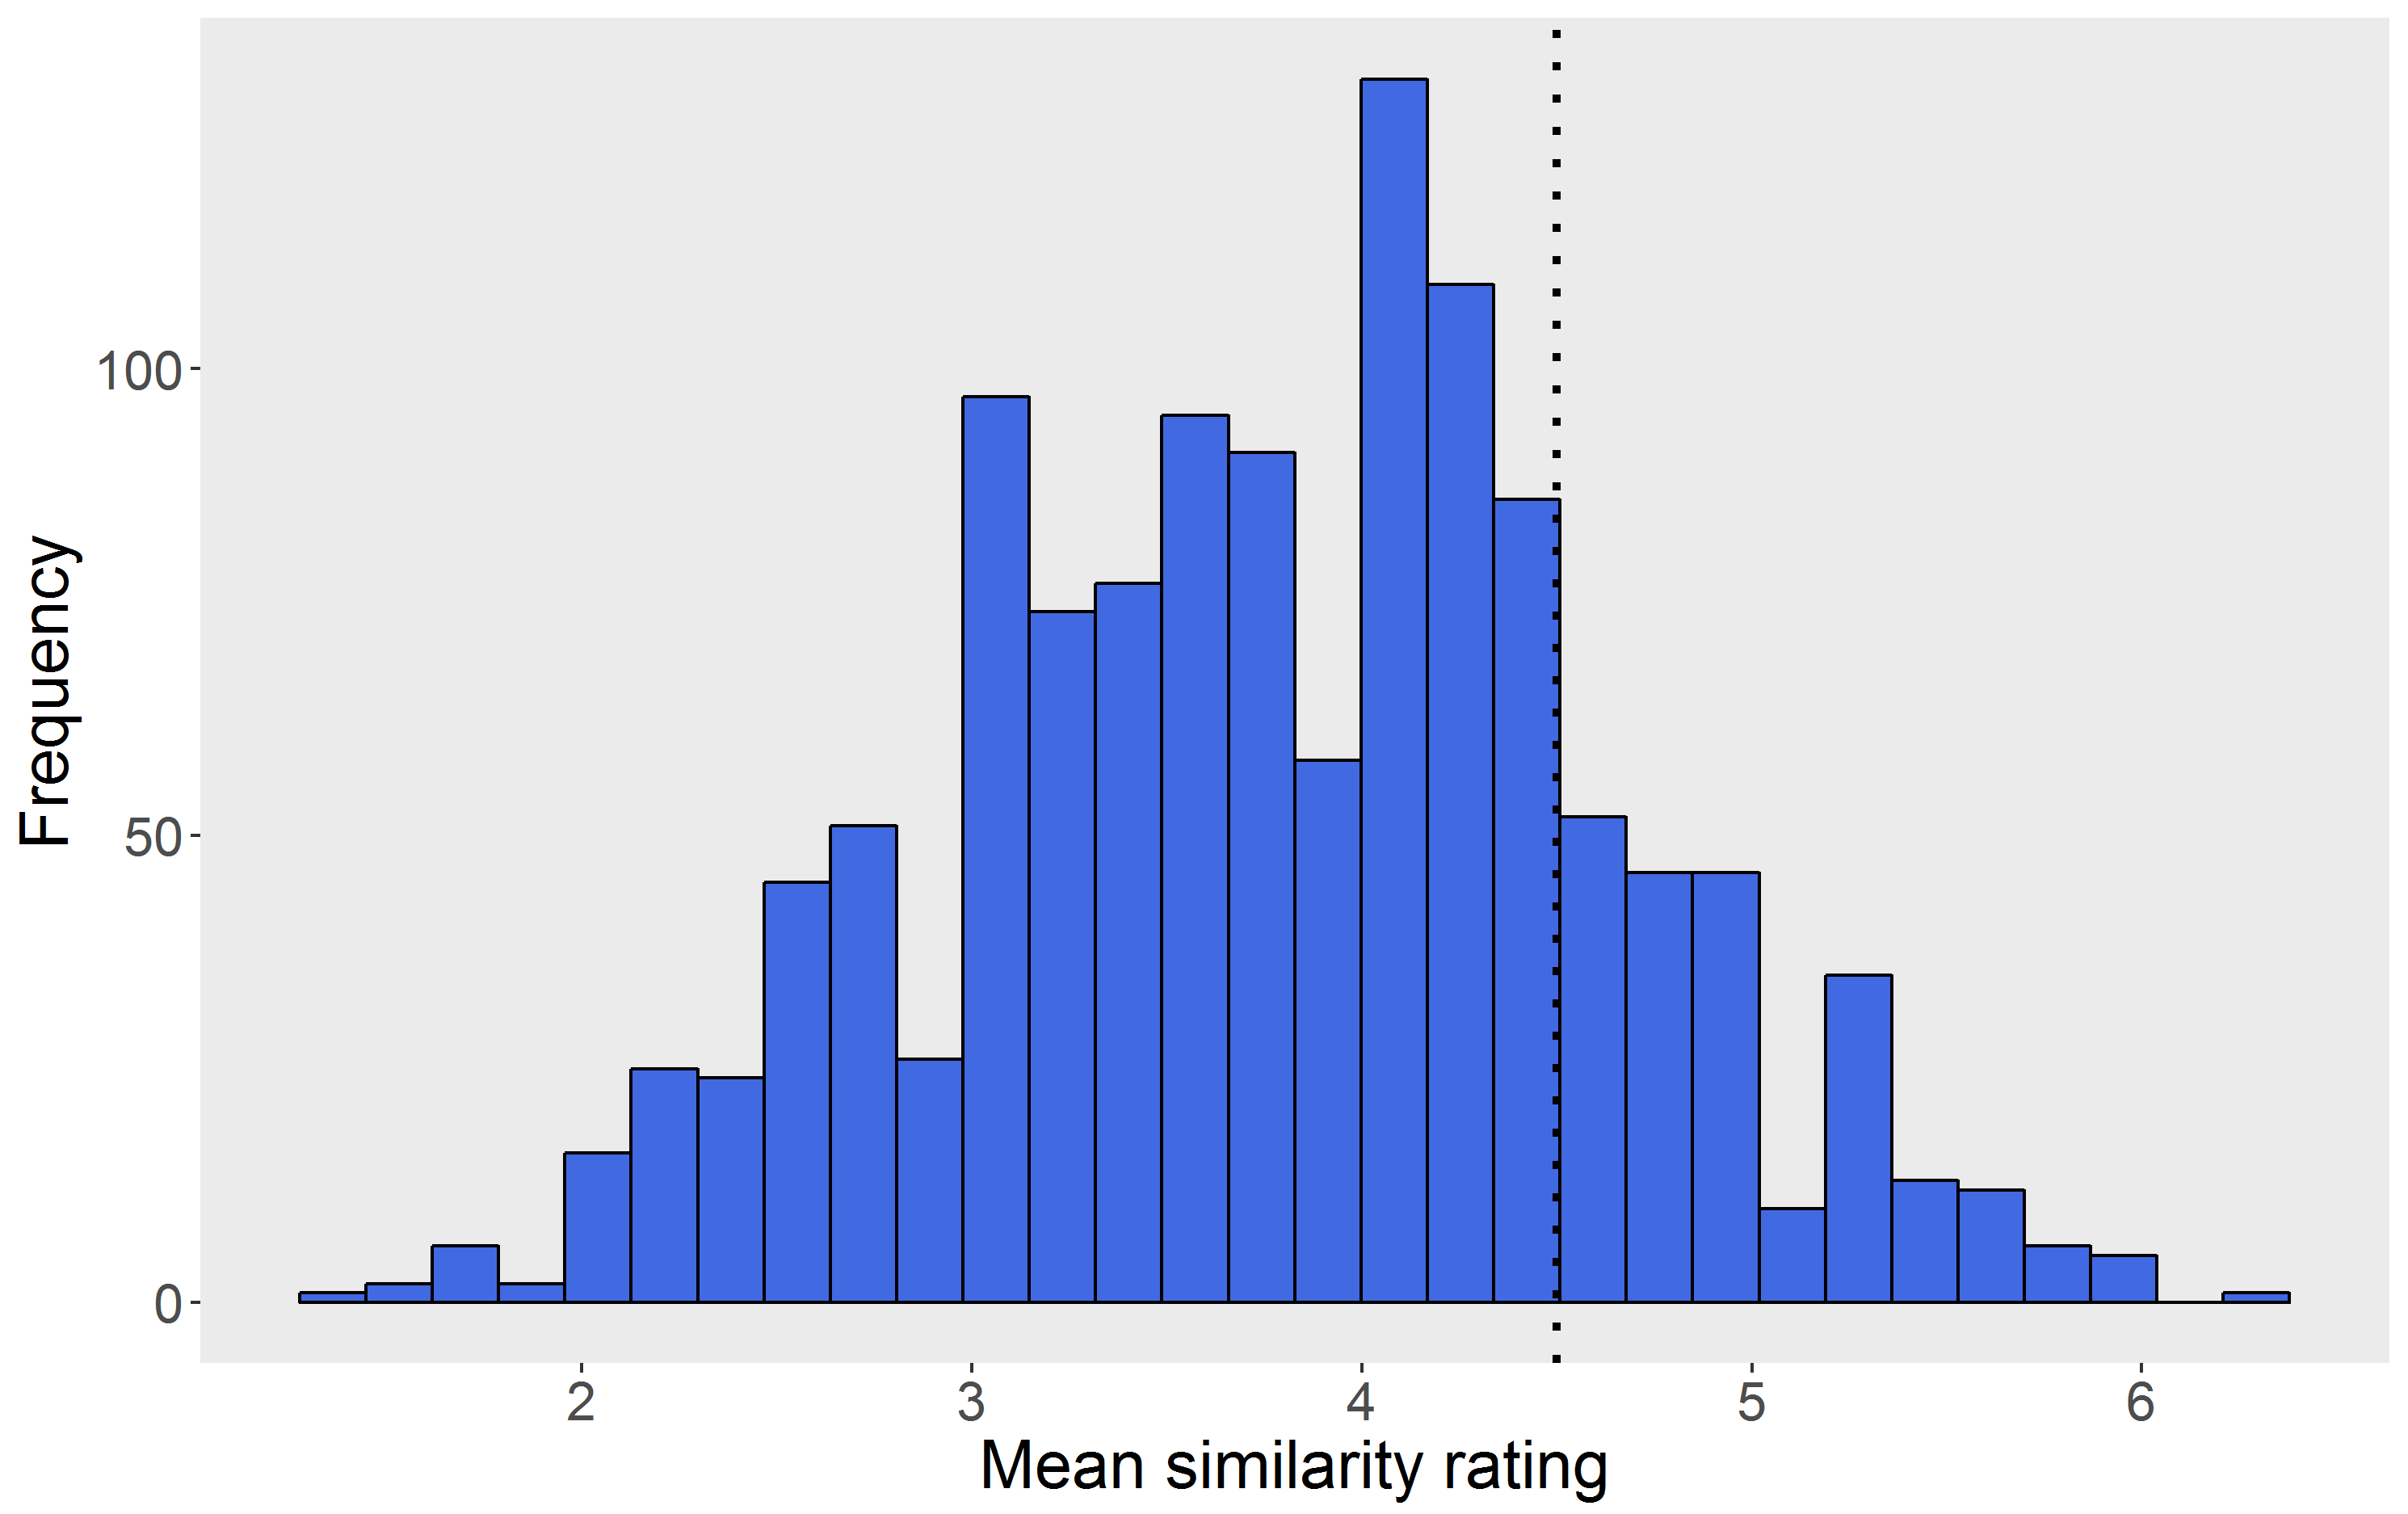
\includegraphics[width=0.9\textwidth]{exp2_pilot.png}
\label{fig:exp2_pilot}
\end{figure}

Once we had a sufficient number of movie pairs that we believed were reasonably similar, the next step in creating the quadruplets was to create target-competitor pairs. To do this, we first created a target-decoy pair by target-decoy pair matrix (253x253), where each cell was the number of overlapping genre categories between the two movie pairs. For example, considering the comparison between target-decoy candidate 1 (consisting of movie A and movie B) and target-decoy candidate 2 (consisting of movie C and movie D), we summed the number of genre overlaps between movies A-C, A-D, B-C and B-D.

 Then we created the quadruplets by combining each target-decoy pair with all the target-decoy pairs that it had no common genre categories with, and taking the unique combinations of the four movies. This resulted in 20,022 quadruplets, created from 231 unique movies.


\subsubsection{Experimental procedure}

The experimental procedure was almost identical to the one described in Experiment 1 (see section \ref{experiment_proced}). We first asked participants to provide preference ratings for 231 movies and specify whether they have seen the movies. After we collected ratings data for the next 50 participants, we identified the quadruplets in which 1) all the movies have either been seen or not seen, 2) the two targets had the same rating and 3) the rating difference between the two targets and their respective decoys were at least 3. Using the same sequential selection procedure (using the sum of the two similarity rating as an indicator for the quality of the choice set), we then obtained a subset of these quadruplets with unique target and competitor movies. We invited back those participants for whom we could create at least three quadruplets.

After the choice stage, we asked each participant to give similarity ratings for each target-decoy and target-competitor pair they encountered in the previous stage. While asking participants to rate the similarity of all target-decoy and target-competitor pairs is costly and time-consuming, this information enabled us to account for individual heterogeneity in similarity perception and making sure that our choice triplets represented an attraction effect choice situation for each participant. 

 We recruited 297 participants using Prolific Academic. Out of the 297 participants that completed part 1, we could create at least one quadruplet that included movies that had either been all seen or not seen for 249 participants, and for 179 of these participants we could create at least 3 quadruplets. Out of the 179 participants who were invited back, 152 took part in the second stage of the experiment.  

\subsubsection{Exclusion criteria}

 We used the same exclusion criteria described in section \ref{exclusion_ref}. After we applied these exclusion criteria to our sample of 152 people, we had choice data from 135 participants.

\subsection{Results}

 Figure \ref{fig:exp2_hist} shows the distribution of the proportion of participants by the number of choice trials. Similarly to Experiment 1, all participants completed an even number of choice trials, the lowest number of choice trials was 6, and the highest was 54. The average number of trials was 16, and 84\% of people were presented with at least 8 choice trials. 
\begin{figure}[htb!]
\centering
\captionsetup{justification=centering}
\caption{Distribution of the proportion of participants by number of choice trials in
Experiment 2.}
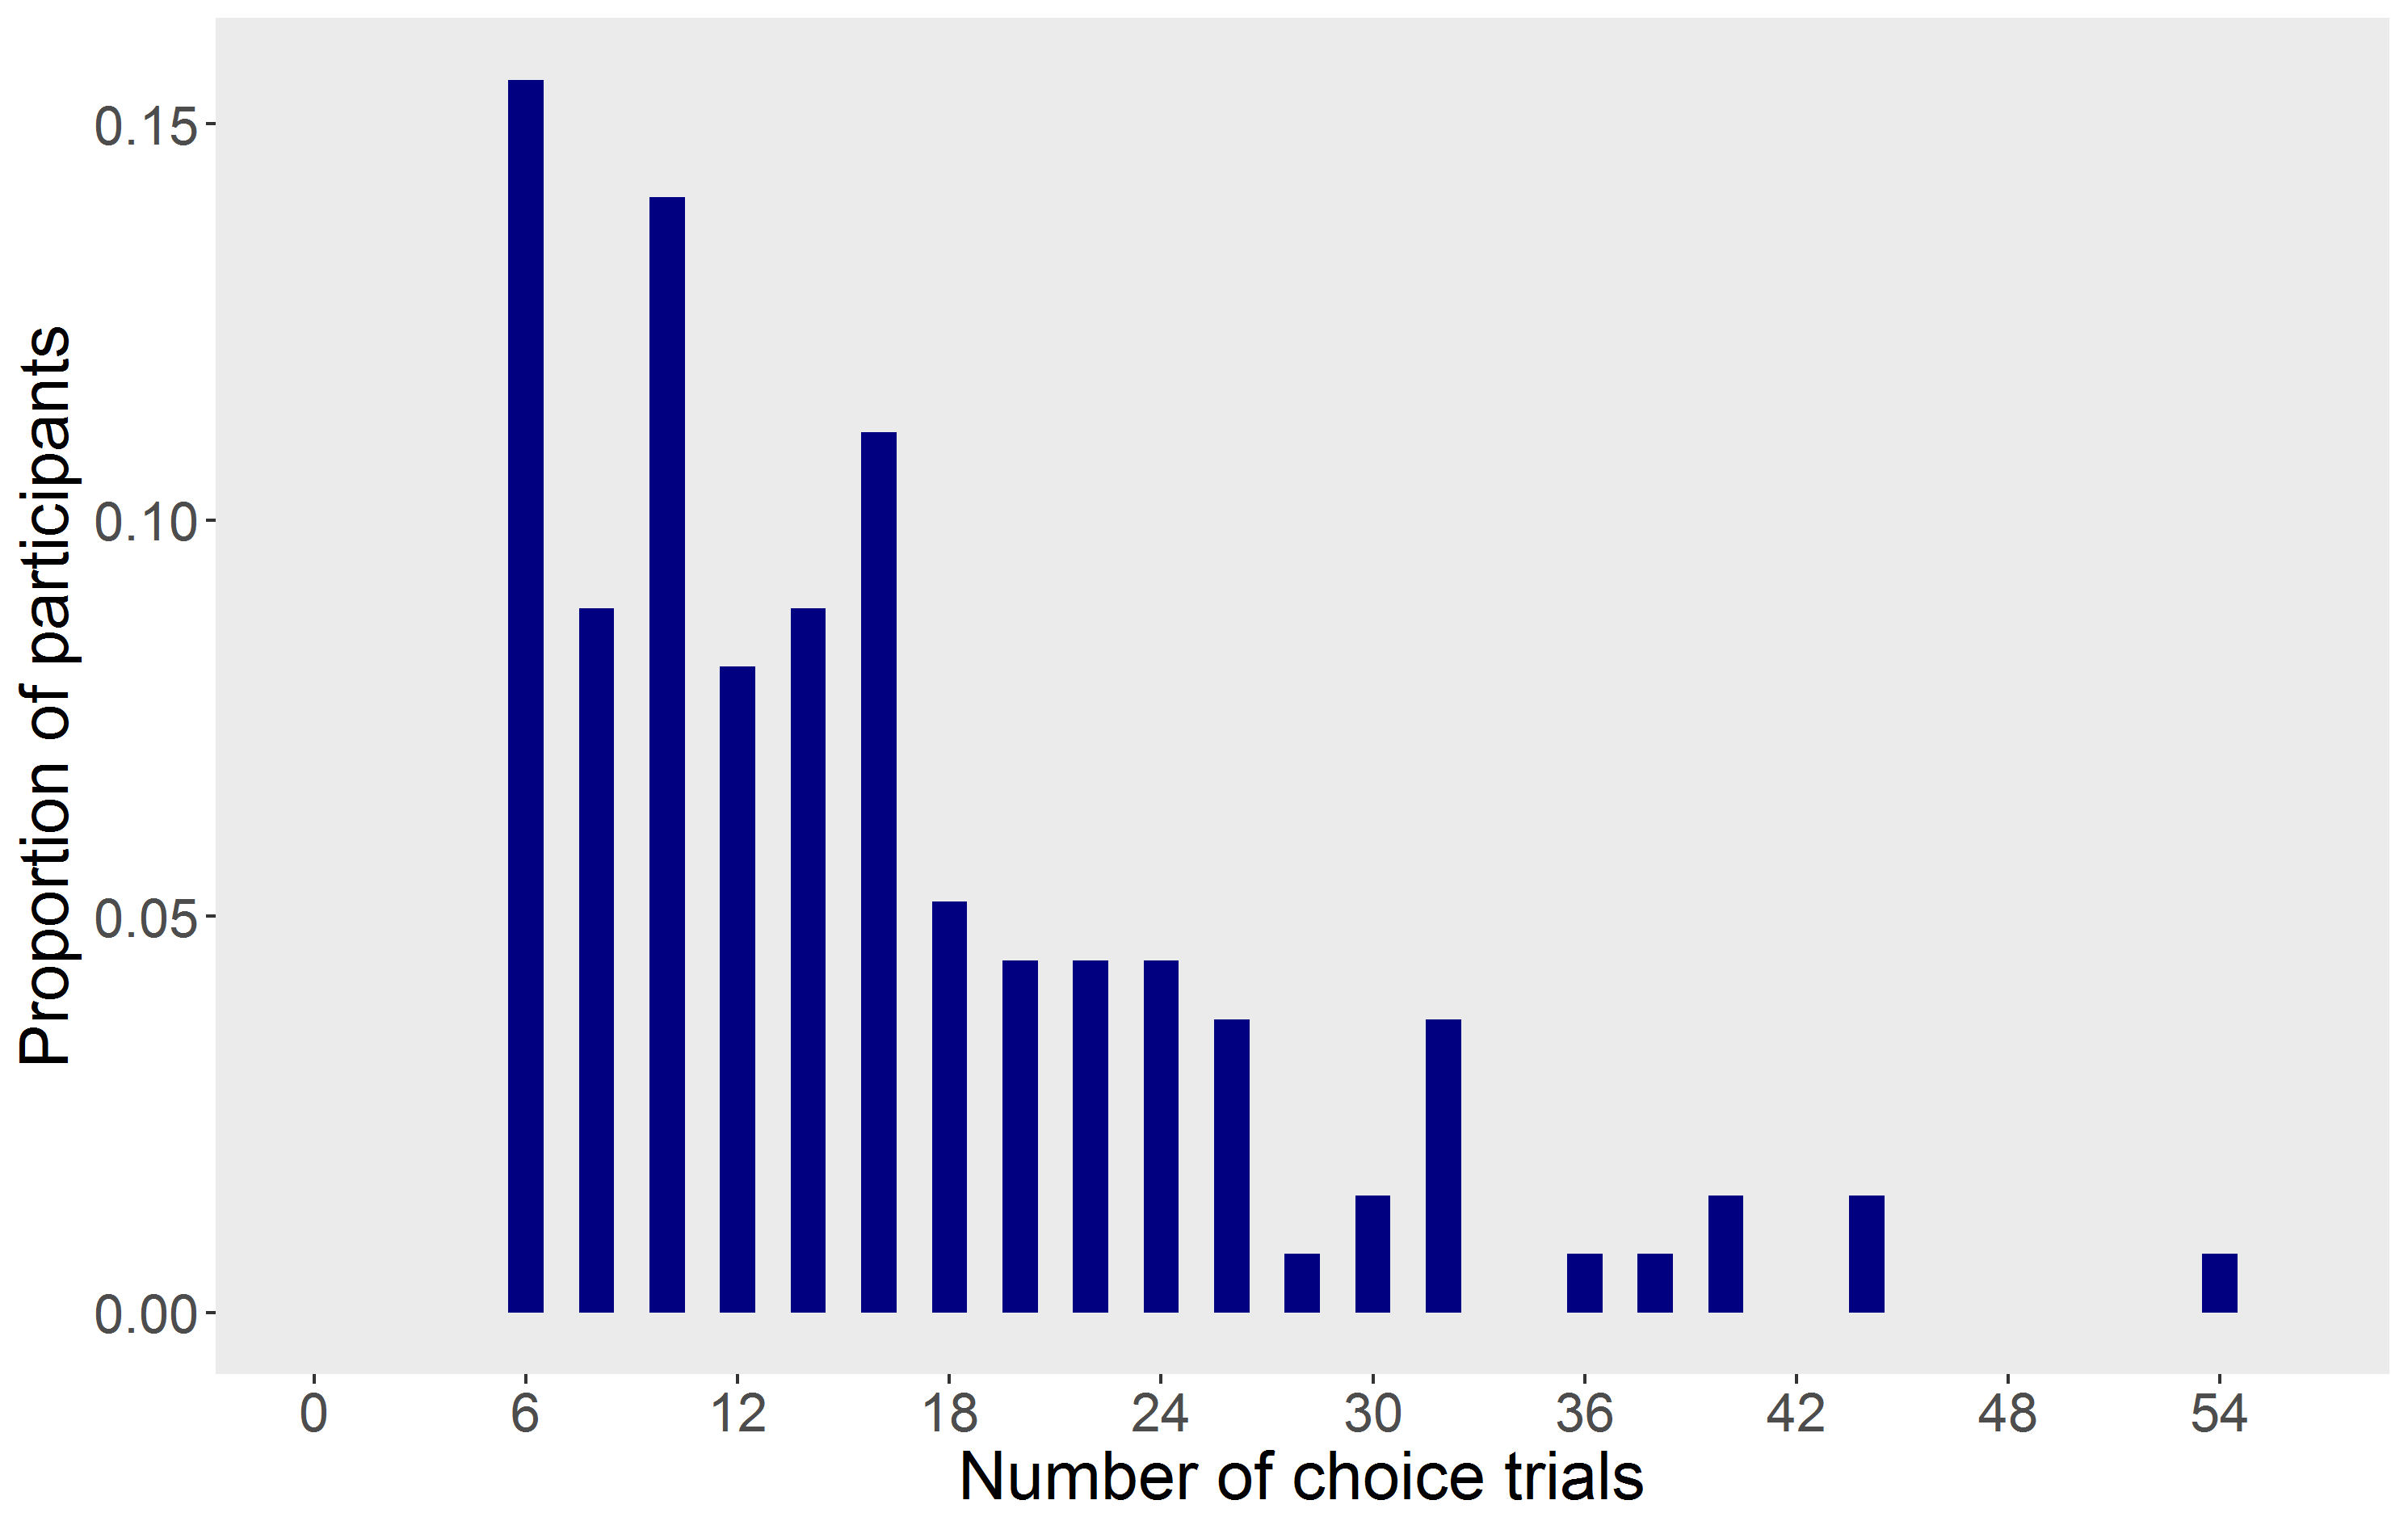
\includegraphics[width=0.8\textwidth]{exp2_hist.png}
\label{fig:exp2_hist}
\end{figure}
 
\begin{figure}[htb!]
\centering
\captionsetup{justification=centering}
\caption{Distribution of the proportion of participants by proportion of trials where the
decoy was chosen in Experiment 2.}
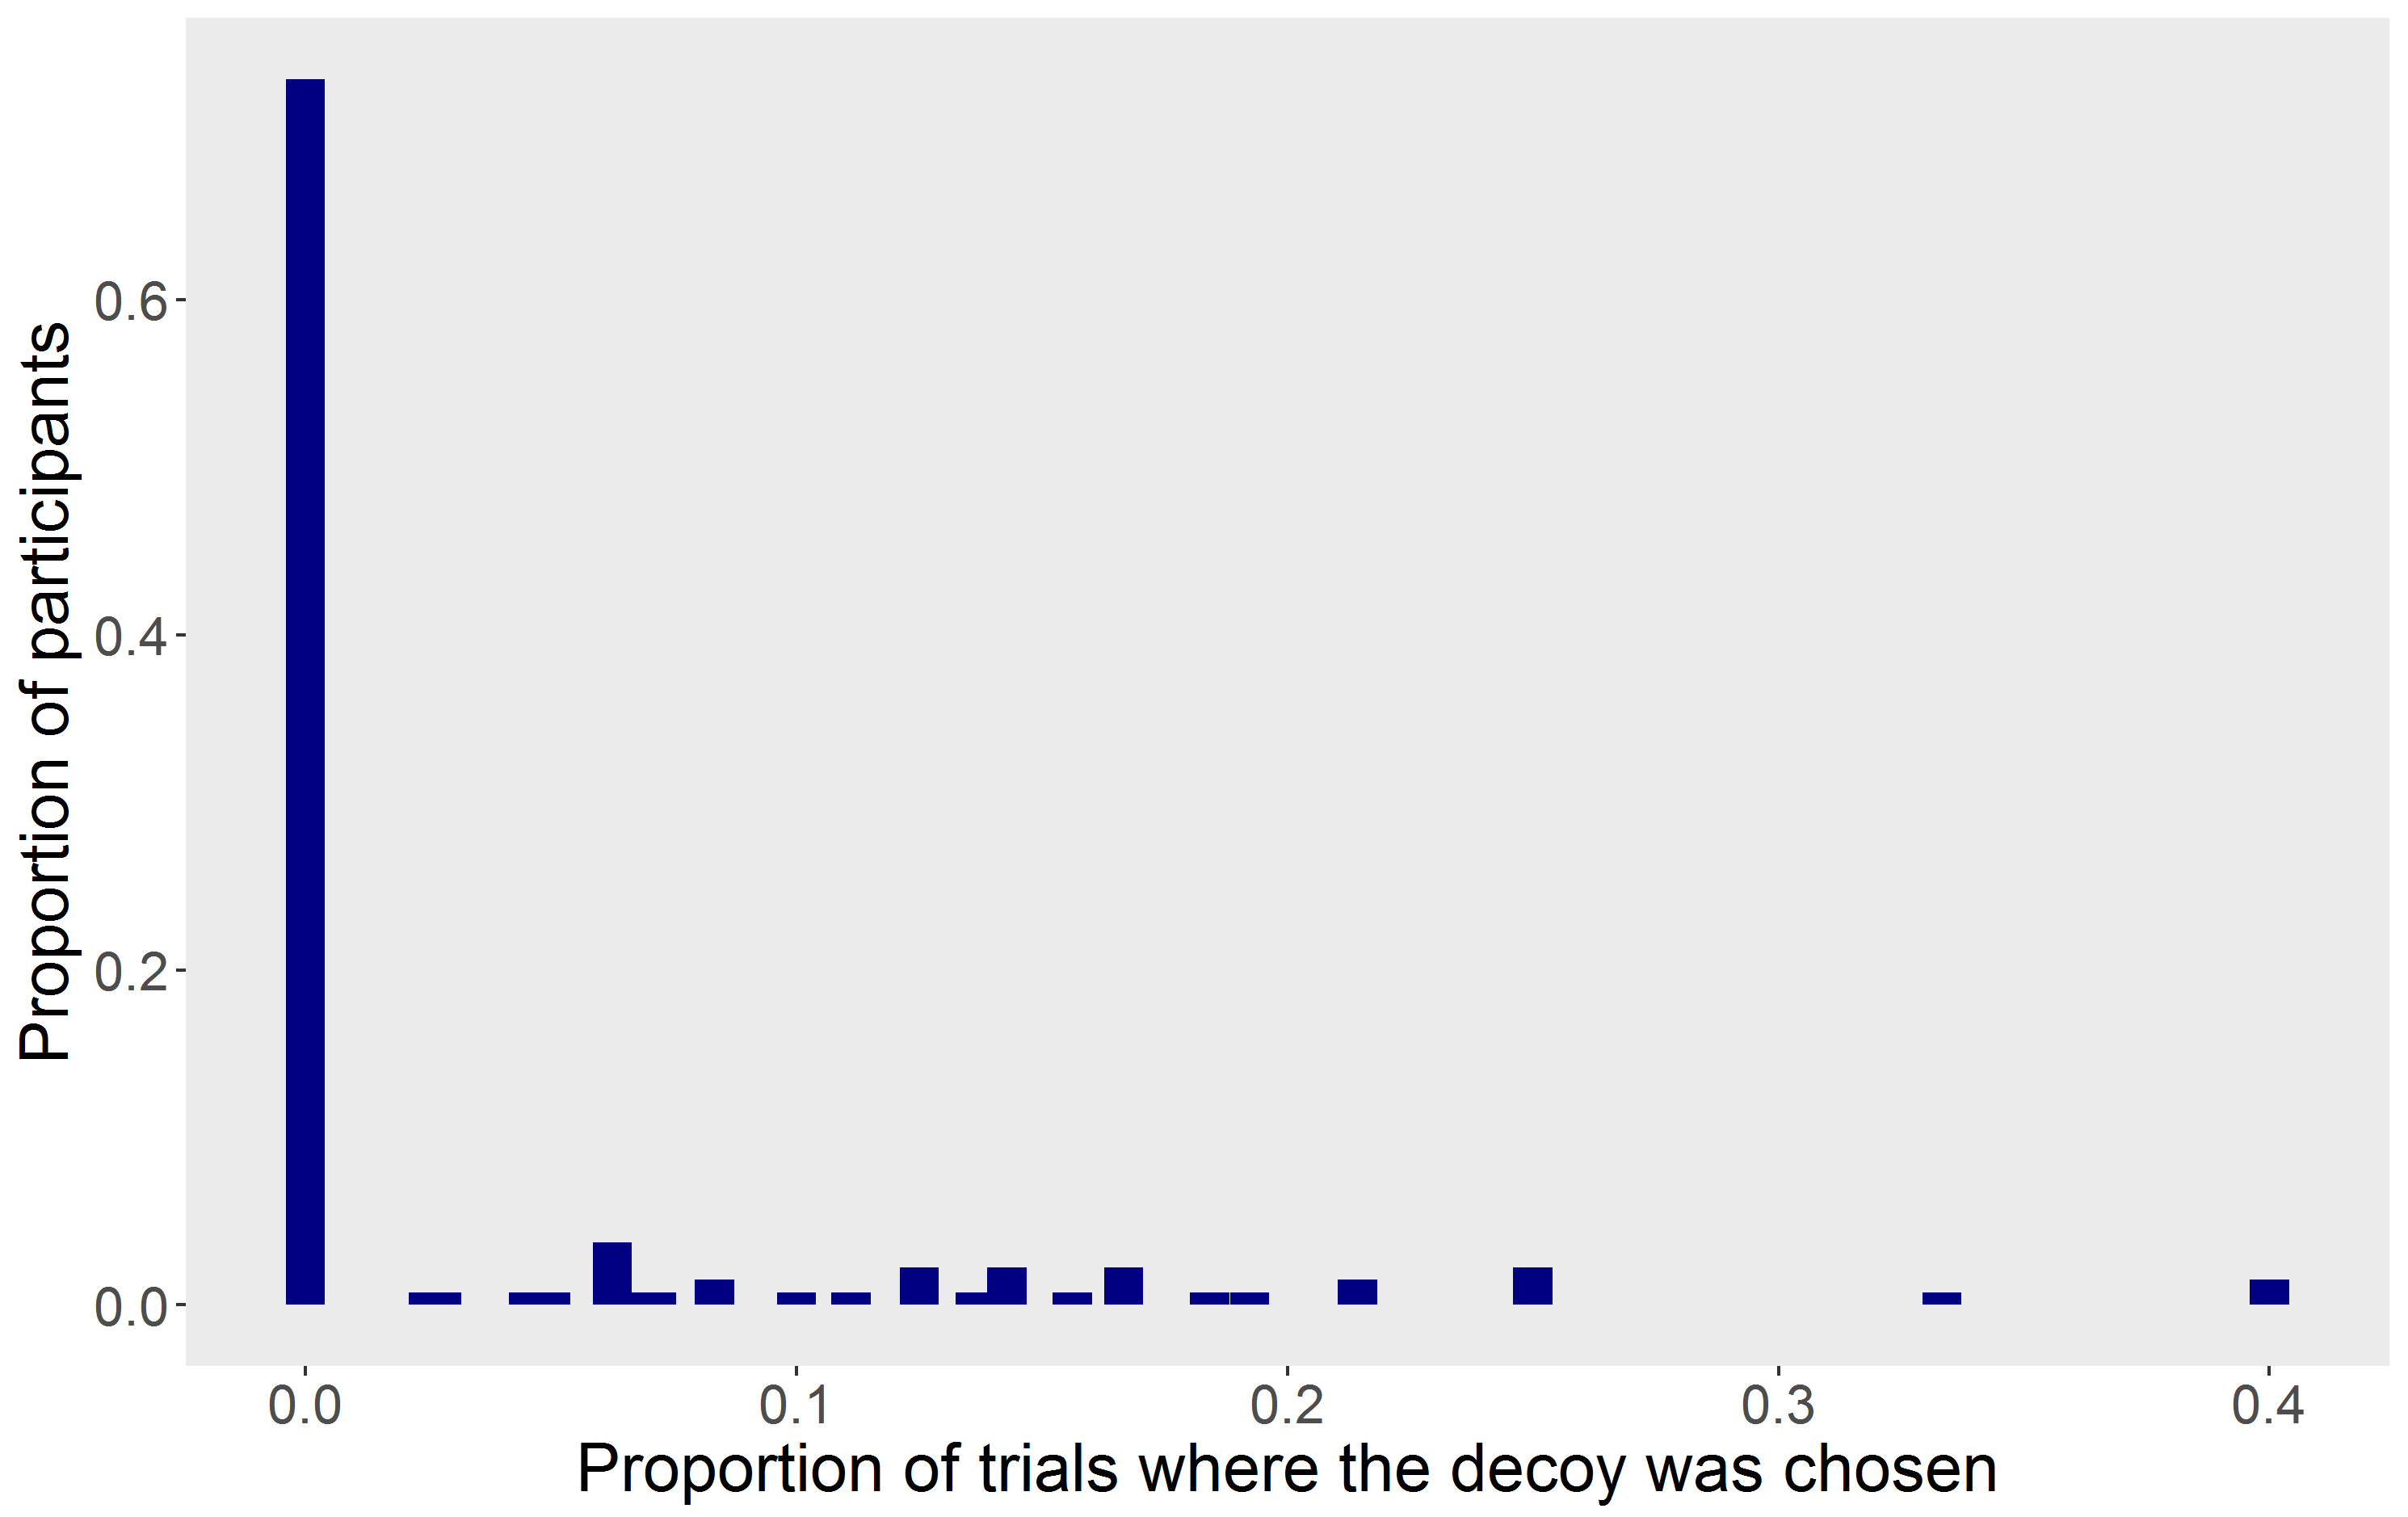
\includegraphics[width=0.8\textwidth]{exp2_decoytrials.png}
\label{fig:exp2_decoytrials}
\end{figure}

Figure \ref{fig:exp2_decoytrials} shows that similarly to Experiment 1, the decoy was again rarely chosen. In fact, 72\% of the participants have never chosen it, and only 2\% of people have chosen it in more than 25\% of the trials. This indicates that people were again able to identify the dominated decoy in the choice stage. 

Before analysing choice behaviour, it is instructive to plot the target-decoy and target-competitor similarity rating distributions, to see if we managed to create more similar target-decoy pairs in Experiment 2.  Figure \ref{fig:exp2_similarityratings} shows these distributions, and we can see that the overwhelming majority of target-competitor pairs were perceived as not similar, while the majority of target-decoy pairs were perceived as similar, which shows that we indeed managed to improve the perceived similarity of the target-decoy pairs.

\begin{figure}[htb!]
\centering
\captionsetup{justification=centering}
\caption{Distribution target-competitor and target-decoy similarity ratings from Experiment 2.}
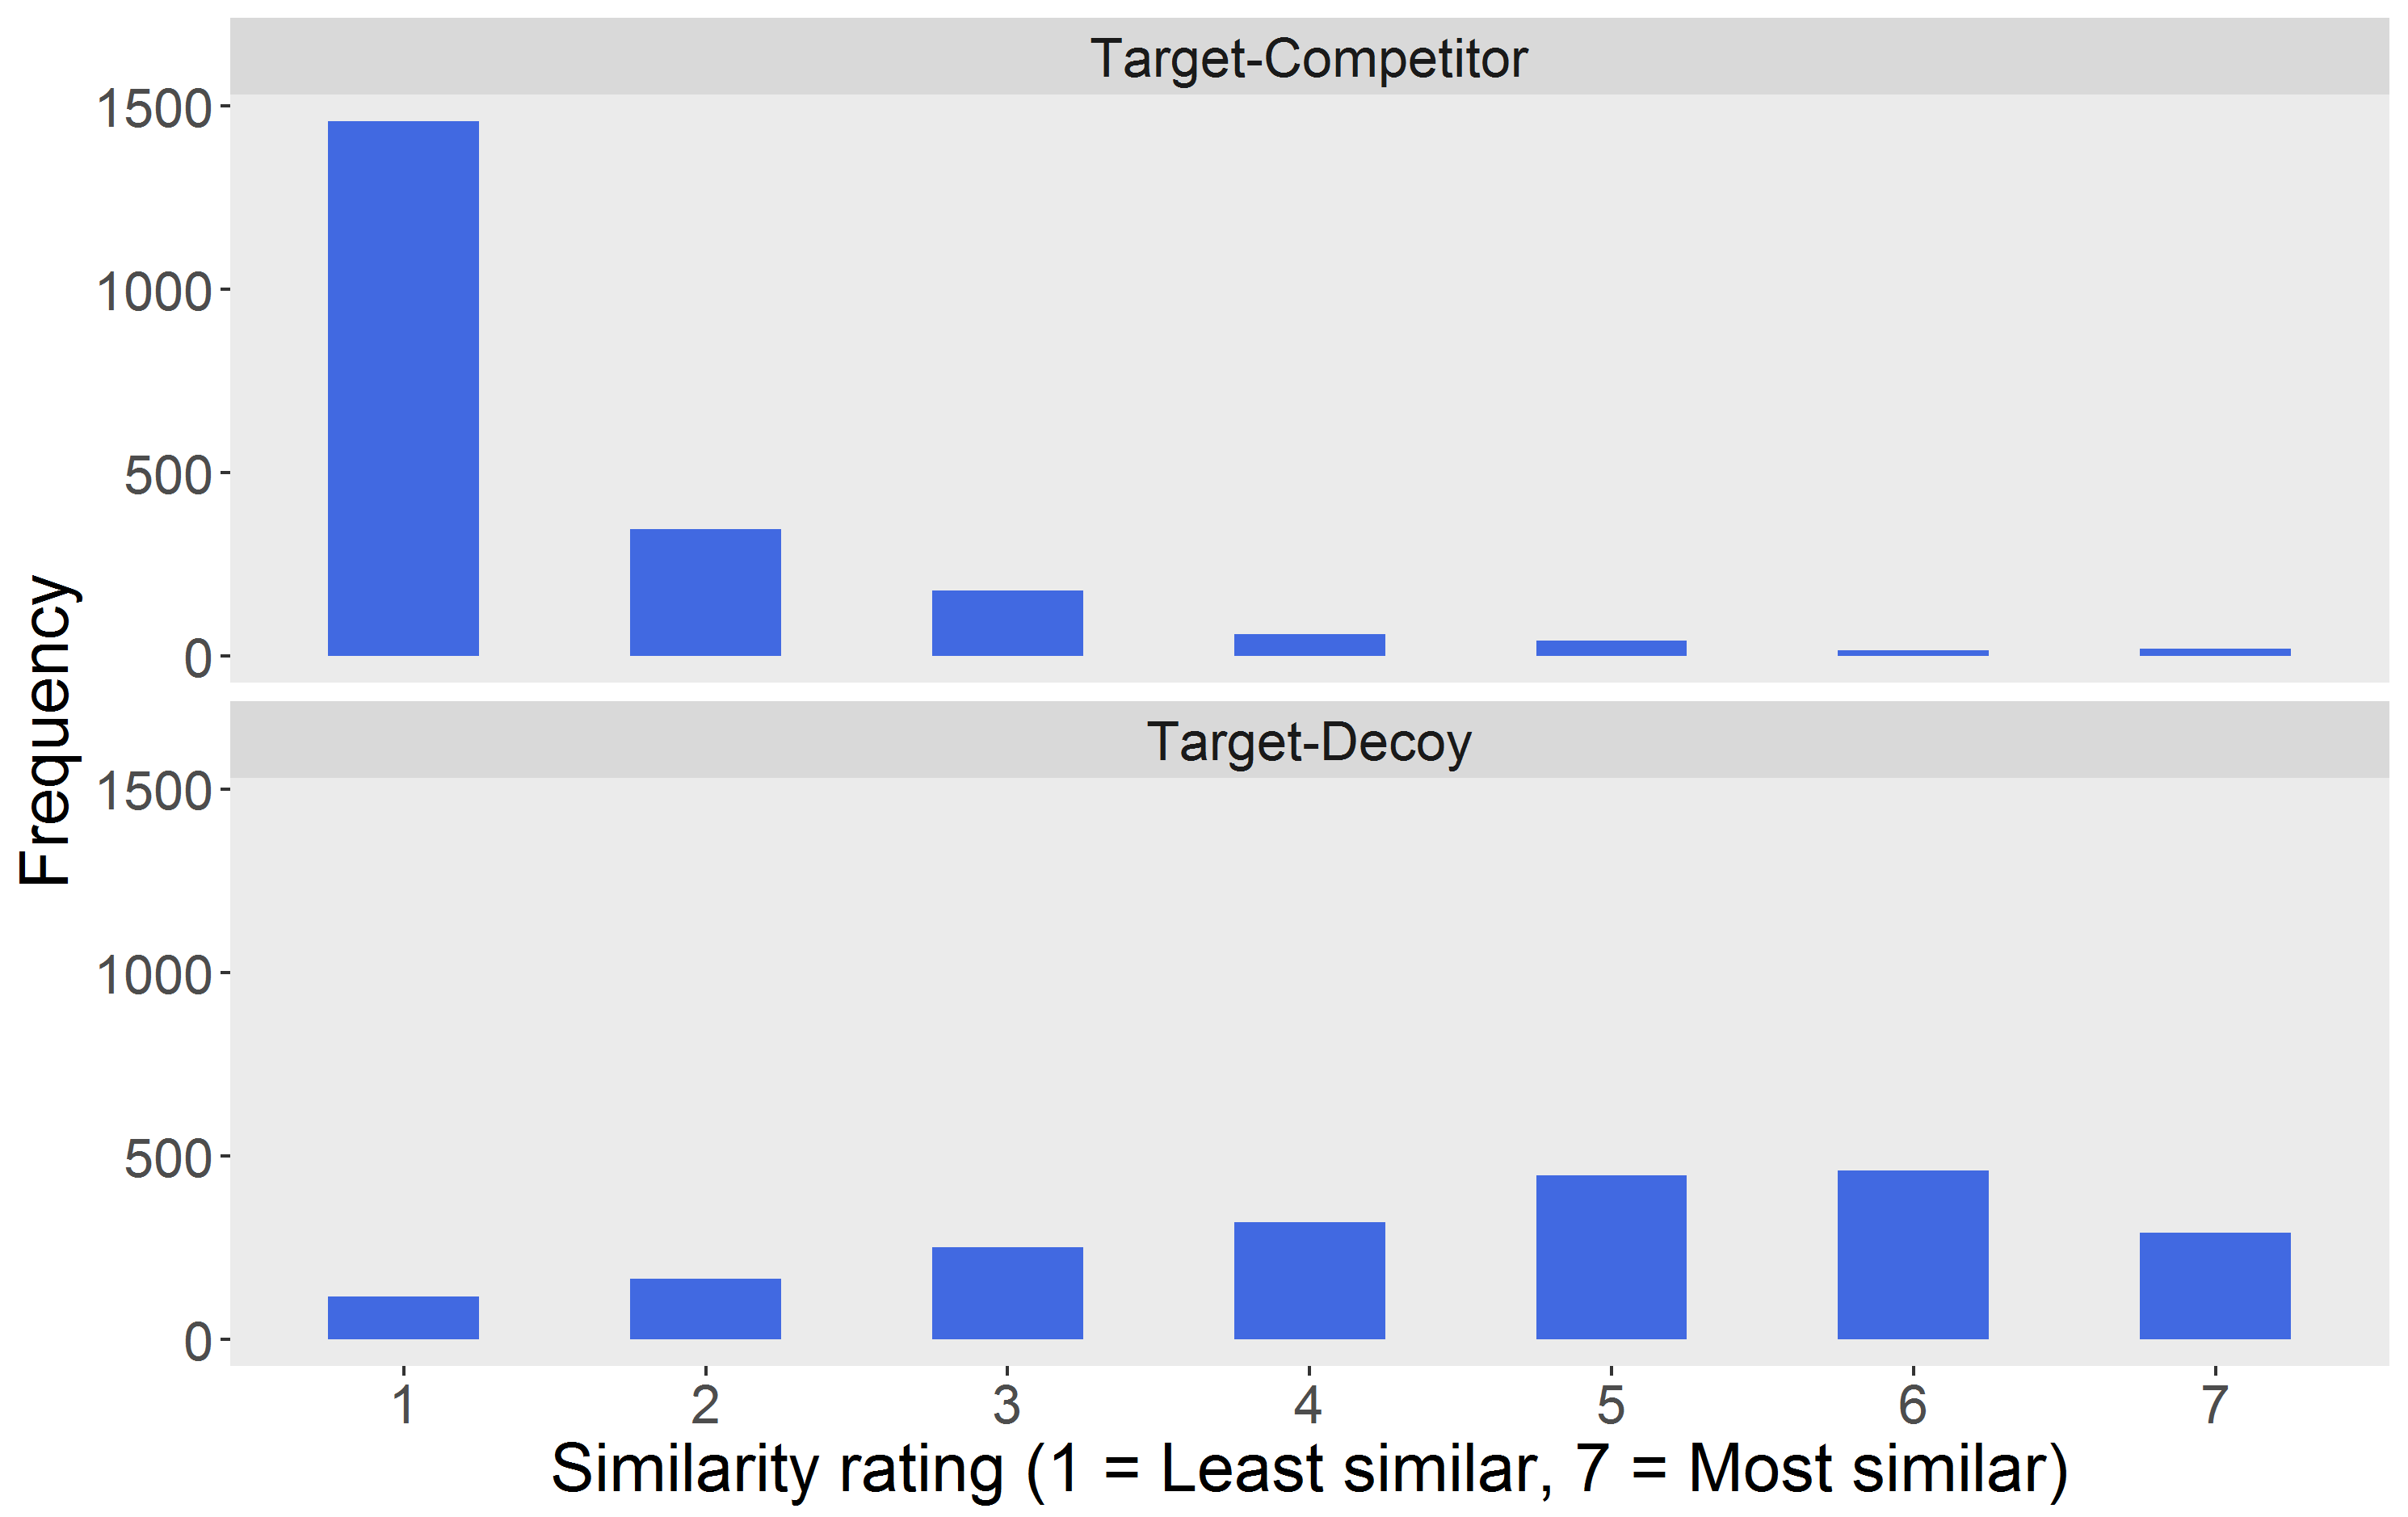
\includegraphics[width=0.8\textwidth]{exp2_similarityratings.png}
\label{fig:exp2_similarityratings}
\end{figure}


To test for the presence of the attraction effect, we again conducted a one-sample t-test to test the hypothesis that the mean of the proportion of trials where the target was chosen  is above 0.5 (indicating an increased likelihood of choosing the target item). The results are very similar to those from Experiment 1: we again found no evidence for the attraction effect (M = 0.5, SD = 0.07), t(134) = -0.44, p = .669. Figure \ref{fig:exp2_res} shows the distribution of the proportions of trials where the target was chosen, which again indicates that participants were indifferent between the target and the competitor, M = 0.5, 95\% CI [0.49, 0.51].

\begin{figure}
\centering
\captionsetup{justification=centering}
\caption{Proportion of trials where the decoy was chosen in Experiment 2. Each dot is a participant and the red dot and error bars show the bootstrapped mean and 95\% CIs.}
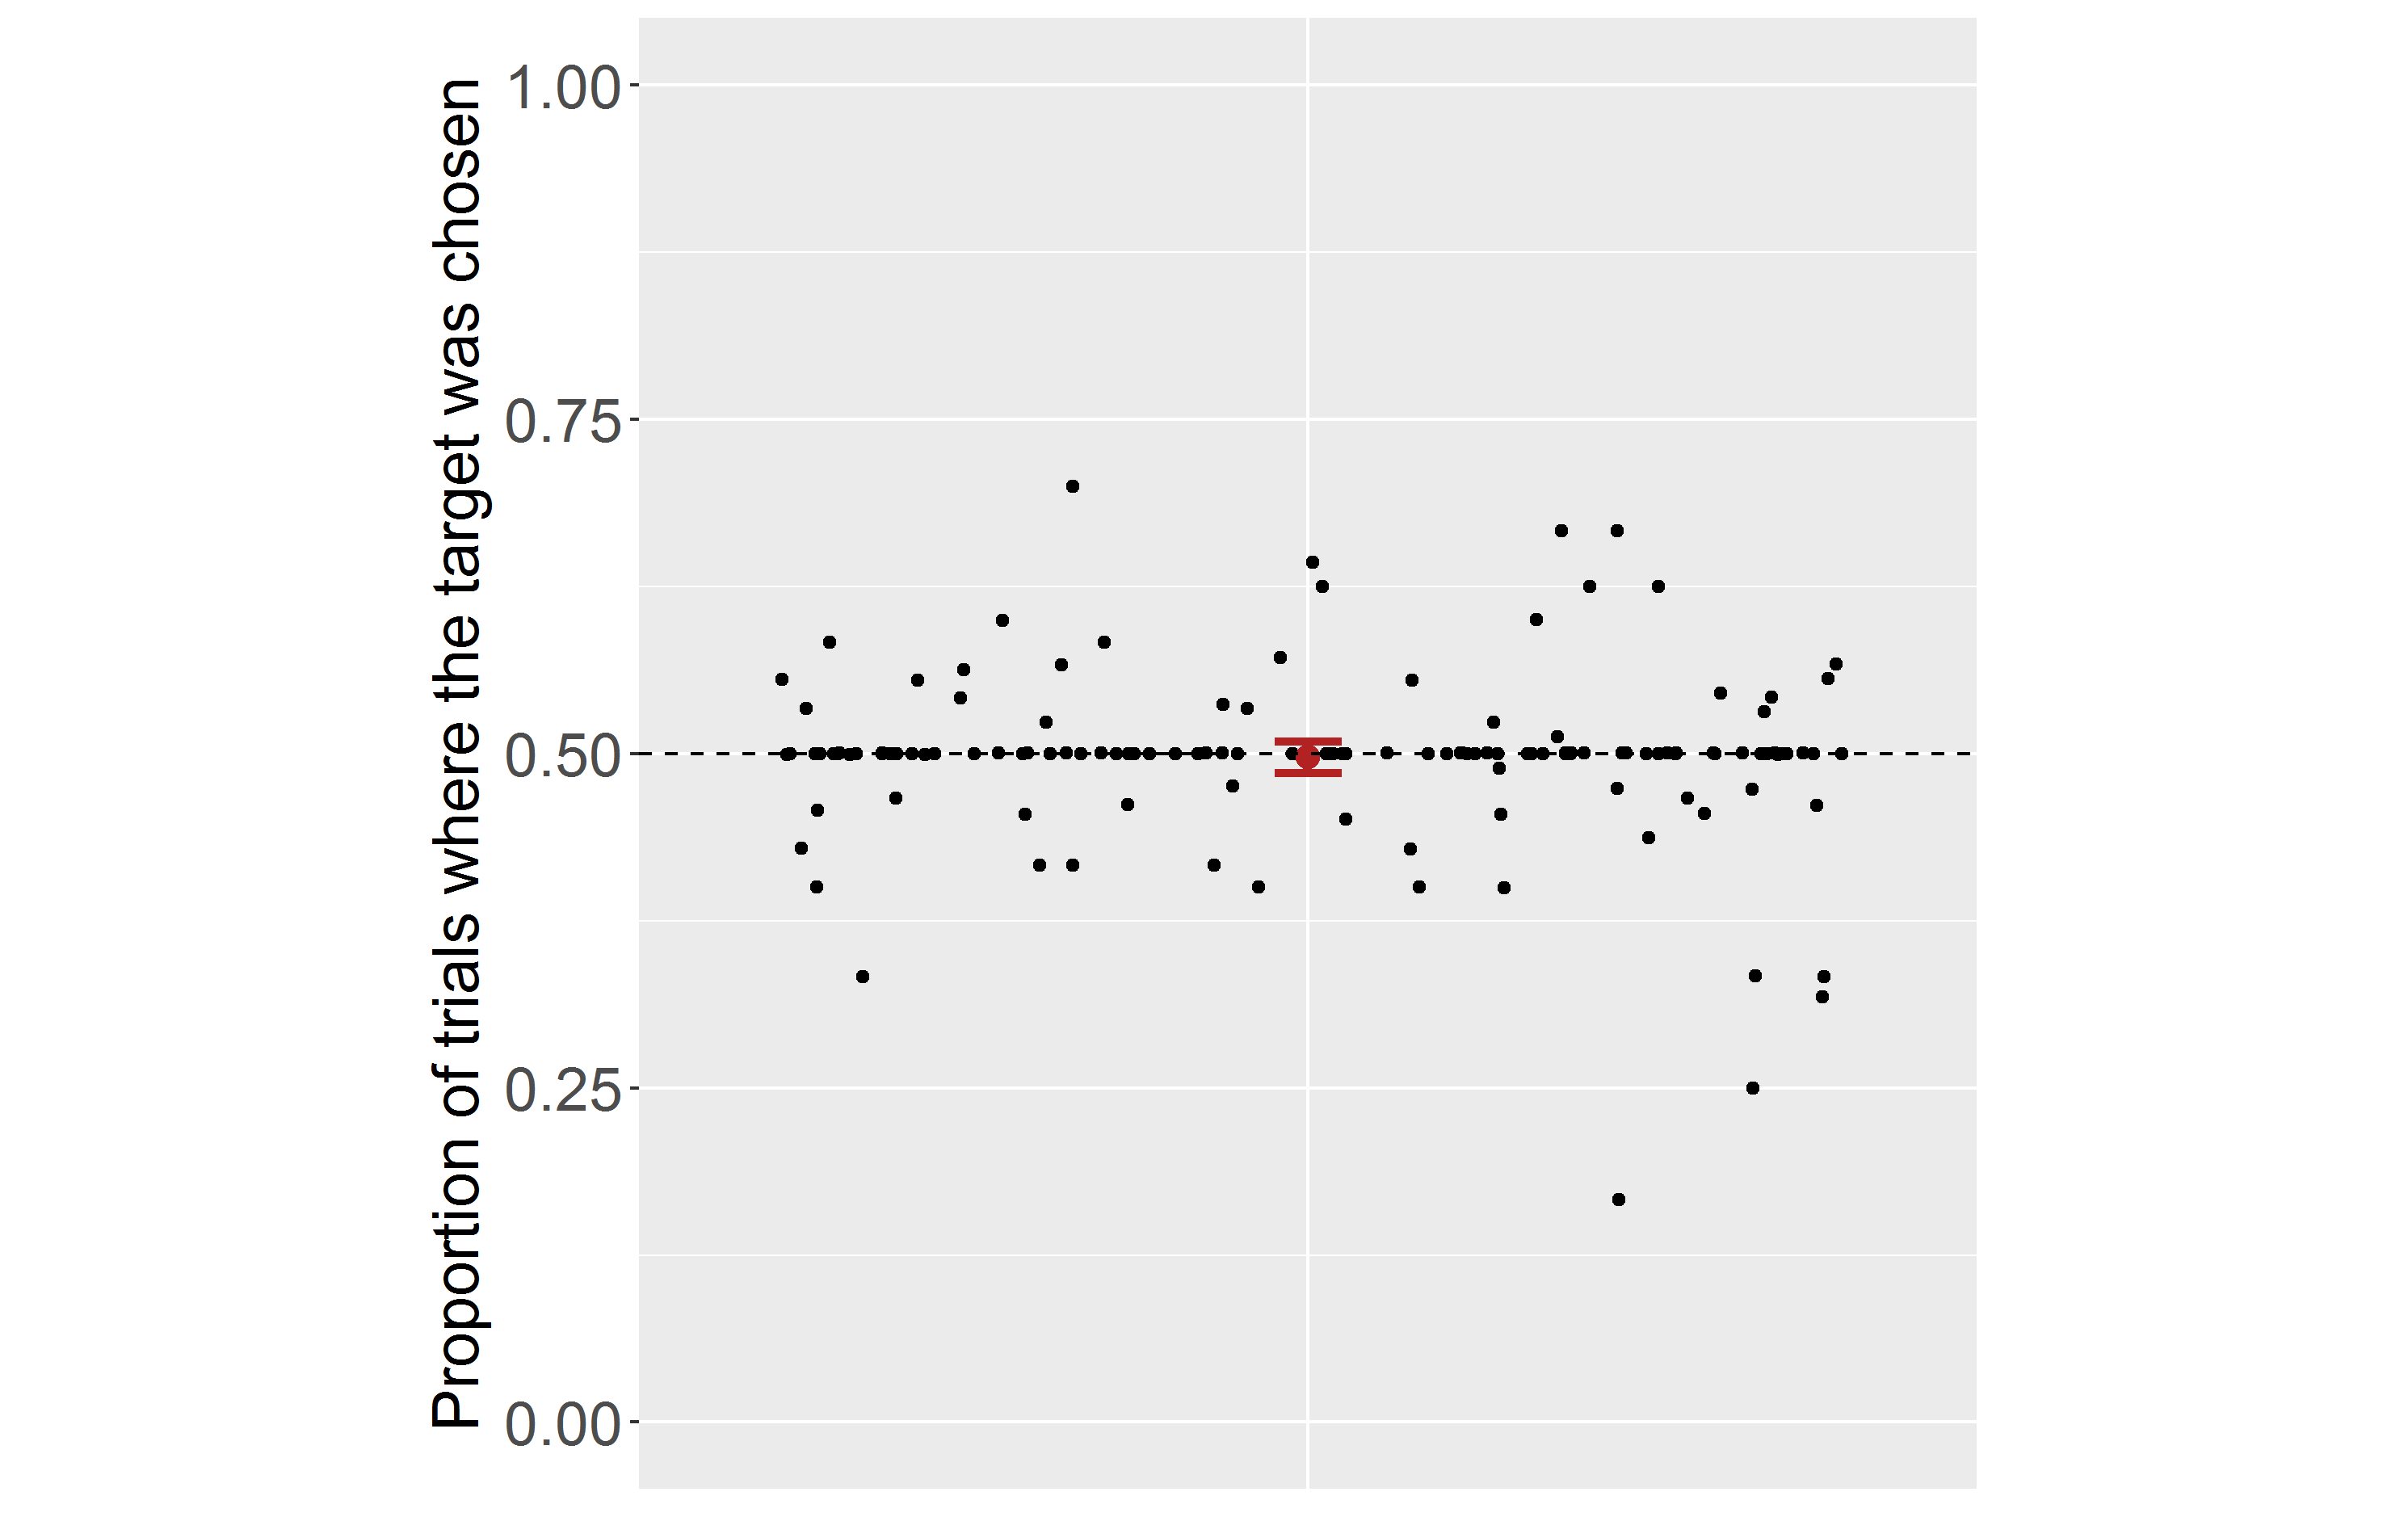
\includegraphics[width=0.8\textwidth]{exp2_res.png}
\label{fig:exp2_res}
\end{figure}



As specified in our pre-registered analysis plan, we also ran a mixed effects logistic regression with subject-specific intercept to investigate how the target-decoy and target-competitor similarity ratings and familiarity of with the movies affect the likelihood of choosing the target. Table \ref{latentattr_exp2reg} shows the results from this regression, where contrary to our expectations, none of the explanatory variables seem to modulate the strength of the attraction effect. 

\begin{table}[!htbp] \centering 
\captionsetup{justification=centering}
  \caption{Odds-ratios and 95\% CIs from a mixed-effects logistic model with subject-specific intercepts, Experiment 2. (T - Target, C - Competitor, D - Decoy)} 
  \label{latentattr_exp2reg} 
\resizebox{9cm}{!}{\begin{tabular}{@{\extracolsep{5pt}}lc} 
\\[-1.8ex]\hline 
\hline \\[-1.8ex] 
 & \multicolumn{1}{c}{\textit{Dependent variable:}} \\ 
\cline{2-2} 
\\[-1.8ex] & Target chosen \\ 
\hline \\[-1.8ex] 
 Seen all & 1.122 (0.731, 1.729) \\ 
  TC similarity rating & 0.967 (0.872, 1.073) \\ 
  TD similarity rating & 0.926 (0.835, 1.027) \\ 
  TD rating difference & 0.935 (0.837, 1.044) \\ 
  Intercept & 1.062 (0.598, 1.882) \\ 
 \hline \\[-1.8ex] 
Observations & 1,541 \\ 
Log Likelihood & $-$1,064.822 \\ 
Akaike Inf. Crit. & 2,141.644 \\ 
Bayesian Inf. Crit. & 2,173.686 \\ 
\hline 
\hline \\[-1.8ex] 
\textit{Note:}  & \multicolumn{1}{r}{$^{*}$p$<$0.1; $^{**}$p$<$0.05; $^{***}$p$<$0.01} \\ 
\end{tabular}}
\end{table}


We can again estimate the probability of choosing the target in an "ideal" attraction effect scenario, where the target-decoy pair is perceived as the most similar, whereas the target-competitor pair is perceived as the least similar. This predicted proportion\footnote{Based on a logistic regression without mixed effects.} is again only 41\%, 95\% CI [31, 52], showing that even when the target-decoy and target-competitor pairs are perceived as very similar/different, we do not see an increased tendency to choose the target (if anything, we see a slight tendency to choose the competitor).

\subsection{Discussion}

Experiment 2 aimed to test the attraction effect with complex, naturalistic stimuli, while accounting for the methodological shortcomings of Experiment 1. Based on the results from Experiment 1, we hypothesized that the we did not find the attraction effect in Experiment 1 due to the fact that participants generally did not perceive the target-decoy pairs as similar.

For this reason, in Experiment 2, we used a rich set of genre information to create similar movie pairs. In addition, we collected similarity ratings on each target-decoy and target-competitor pair participants encountered in the choice stage. This allowed us to see how the strength of the attraction effect depends on the perceived similarity of the movie pairs.

The results are broadly similar to those from Experiment 1. That is, we have found that the presence of a dominated decoy does not alter preferences between the target and the competitor (we are 95\% confident that the true proportion of trials where the target was chosen is between 49\% and 51\%). In addition, to our surprise, the tendency to choose the target was not affected by the perceived similarity of the target-decoy and target-competitor pair.

\newpage

\section{General Discussion} 

In Experiment 1 and 2, we investigated the prevalence of the attraction effect in a naturalistic choice context. While previous research had shown that the effect is rather robust in choice tasks where the attributes have a numerical representation, its relevance has been debated in choices that involve naturalistic options.

To conduct a test of the attraction effect using complex stimuli, we used movie posters as real-world choice options to create target-competitor-decoy choice triplets. In Experiment 1, we did not find any evidence for the attraction effect, but we also found that participants did not perceive our target-decoy pairs as similar, which cast doubt on the validity of our test. To address this problem, we conducted the same test with an improved methodology in Experiment 2. We believe that Experiment 2 is the first rigorous investigation of this research question: we designed it carefully to address all the criticisms raised in connection with the study by \citeauthor{Frederick2014}, where they used similar stimuli.

First, our experimental design ensured participants' indifference between the target and the decoy, maximising the probability that choices will be constructed on the spot (rather than through relying on strong prior preferences), and an attraction effect will occur. While one could argue that mnemonic processes arising from familiarity with the stimuli can alter preferences in the choice stage, we still did not detect an attraction effect when participants were not familiar with the movies. 

Second, we have strong evidence that the dominance relationship was perceived in our experiment. The target-decoy similarity ratings confirmed that our careful target-decoy selection process indeed managed to produce movie pairs that were perceived as similar. In addition, we ensured that the decoy was always rated at least 3 units lower than the target (and the competitor). Accordingly, the decoy was only chosen in 4.3\% of the trials, which clearly shows that participants were able to spot and avoid the dominated alternative.

Third, by creating bespoke choice triplets based on preference ratings, we avoided individual heterogeneity in preferences to act as a potential confound. In addition, we ensured that the decoy is not too desirable in comparison to the target. We also used a strict exclusion criteria to filter out participants who did not take the task sufficiently seriously, and with an average of 16 choice trials per participant we avoided participant fatigue.


Finally, in our analysis we controlled for familiarity with the choice options, perceived similarity of the target-decoy and target-competitor pair, and relative preference between the target and the decoy, but we found that none of these modulated the strength of the attraction effect.

The results from this rigorous test duplicated the findings from Experiment 1: the presence of the decoy in the choice set did not alter preferences between the target and the competitor. Therefore, we can conclude that even when we accounted for the criticisms in connection with \citeauthor{Frederick2014} and \citeauthor{Yang2014}'s studies, we still did not find the attraction effect when options had complex, naturalistic attributes. This illuminates the possibility that the discrepancy stems directly from the stimuli presentation, which might give rise to fundamentally different comparison processes.

Unfortunately, \citeauthor{Frederick2014} did not elaborate on the potential reasons for their results. They briefly conclude that it is the numerical nature of the attribute dimensions that give rise to the attraction effect, but we think this is a simplification. In fact, it has been shown on numerous occasions that the attraction effect is also present in settings where options do not have numerical attributes. 

For example, \citeA{Choplin2005a} have demonstrated the effect in a similarity judgment task with unidimensional stimuli (by varying the aspect ratio of circles and the length of lines). \citeA{Maylor2007} have found the attraction effect in a memory judgment task.  \citeA{Farmer2015} have demonstrated the effect in motor planning decisions. In addition, the attraction effect has also been found in experiments using perceptual stimuli. In \citeauthor{Trueblood2013}, participants were presented with rectangles of differing height and width, and had to select the rectangle with the largest area. Other studies have used the same rectangle stimuli and found the attraction effect in children \cite{Zhen2016} and monkeys \cite{Parrish2015}.

 Interestingly, \citeauthor{Frederick2014} presented the only experiment we know about that did not find the attraction effect using \citeNP{Trueblood2013}'s perceptual stimuli. However, important differences exist between the two experimental methodologies, which is reflected by the fact that in \citeauthor{Frederick2014}'s study, the decoy's choice share was double of that reported in \citeauthor{Trueblood2013}'s experiment. Nevertheless, we think replications are key in understanding the boundary conditions of the attraction effect. We are aware of the fact that there is an unfortunate tendency in psychology not to report failed replication attempts \cite{Ingre2015}, which hinders our understanding of how the strength of the attraction effect depends on the stimuli characteristics.

We find these contradictory results interesting, as it illuminates the possibility that it is not the numerical nature of the attribute dimensions, but some other attribute characteristic that underlies the attraction effect. We aim to explore this possibility in Chapter \textcolor{red}{x}.












\bibliographystyle{apacite}

\newpage

\bibliography{refs}

\end{document}
